\documentclass[12pt,a4paper]{article}
\usepackage[margin=25mm,headheight=15pt]{geometry}
\usepackage{fontspec}
\setmainfont{Times New Roman}
\setsansfont{Arial}
\setmonofont{Consolas}

\usepackage{microtype,graphicx,booktabs,array,longtable,calc,float,placeins,needspace}
\usepackage{amsmath,amssymb,xcolor,caption,fancyhdr,titlesec,setspace}
\usepackage[hidelinks,breaklinks=true]{hyperref}
\usepackage{lineno}
\pagestyle{fancy}
\fancyhf{}
\fancyhead[L]{\sffamily\small ChemWorld | Author manuscript}
\fancyhead[R]{\sffamily\small Integrated research draft}
\fancyfoot[C]{\small\thepage}
\renewcommand{\headrulewidth}{0.3pt}
\setlength{\columnsep}{7mm}
\setlength{\parindent}{0pt}
\setlength{\parskip}{4pt}
\setlength{\emergencystretch}{3em}
\setlength{\tabcolsep}{3pt}
\renewcommand{\arraystretch}{1.1}
\clubpenalty=10000
\widowpenalty=10000
\titleformat{\section}{\large\bfseries\sffamily\raggedright}{}{0pt}{}
\titleformat{\subsection}{\normalsize\bfseries\sffamily\raggedright}{}{0pt}{}
\titleformat{\subsubsection}{\small\bfseries\sffamily\raggedright}{}{0pt}{}
\titlespacing*{\section}{0pt}{10pt}{5pt}
\titlespacing*{\subsection}{0pt}{9pt}{4pt}
\captionsetup{font=small,labelformat=empty,justification=justified}
\renewcommand{\topfraction}{.95}
\renewcommand{\bottomfraction}{.9}
\renewcommand{\textfraction}{.04}
\renewcommand{\floatpagefraction}{.75}
\renewcommand{\dbltopfraction}{.95}
\renewcommand{\dblfloatpagefraction}{.75}
\makeatletter\setlength{\@fptop}{0pt}\setlength{\@dblfptop}{0pt}\makeatother
\providecommand{\tightlist}{\setlength{\itemsep}{0pt}\setlength{\parskip}{0pt}}
\providecommand{\pandocbounded}[1]{#1}
\newlength{\cslhangindent}\setlength{\cslhangindent}{1.5em}
\newlength{\csllabelwidth}\setlength{\csllabelwidth}{2em}
\newenvironment{CSLReferences}[2]{\small\setlength{\parindent}{0pt}\setlength{\parskip}{4pt}}{\par}
\newcommand{\CSLBlock}[1]{#1\hfill\break}
\newcommand{\CSLLeftMargin}[1]{\par\noindent\makebox[\csllabelwidth][l]{#1}}
\newcommand{\CSLRightInline}[1]{\parbox[t]{\dimexpr\linewidth-\csllabelwidth\relax}{#1}\par}
\newcommand{\CSLIndent}[1]{\hspace{\cslhangindent}#1}
\hypersetup{pdftitle={Abductive inquiry in autonomous science},pdfauthor={Jiangjie Qiu; Yijun Li; Yaotian Yang; Honghao Chen; Wentao Li; Xiaonan Wang}}
\begin{document}
\doublespacing

\begingroup\singlespacing
{\sffamily\small ARTICLE\hfill 16 October 2026\par}
\vspace{8pt}
{\sffamily\LARGE\bfseries\raggedright\hyphenpenalty=10000 Abductive inquiry in autonomous science\par}
\vspace{8pt}
{\normalsize Jiangjie Qiu\textsuperscript{1,*}, Yijun Li\textsuperscript{1,*}, Yaotian Yang\textsuperscript{1,*}, Honghao Chen\textsuperscript{1}, Wentao Li\textsuperscript{1}, Xiaonan Wang\textsuperscript{1,\textdagger}\par}
{\footnotesize\textsuperscript{1}Beijing Key Laboratory of Artificial Intelligence for Advanced Chemical Engineering Materials, State Key Laboratory of Chemical Engineering and Low-Carbon Technology, Department of Chemical Engineering, Tsinghua University, Beijing 100084, China.\par}
{\footnotesize * Jiangjie Qiu, Yijun Li and Yaotian Yang contributed equally.\par}
{\footnotesize $\dagger$ Correspondence: \href{mailto:wangxiaonan@tsinghua.edu.cn}{wangxiaonan@tsinghua.edu.cn}.\par}
\vspace{6pt}
{\sffamily\footnotesize Figures 2, 5 and 6 retain quantitative artwork. Other figures are labelled ImageGen concepts or data previews; generated geometry is illustrative.\par}
\vspace{8pt}
\endgroup
\textbf{Autonomous science requires agents to develop explanations that can guide and withstand experimental inquiry. How such explanations emerge from an agent's own research remains poorly understood. Here we introduce ChemWorld, programmable chemical worlds that combine autonomous experimentation with independent control of underlying laws and supplied information. Across chemical systems, model configurations and repeated investigations, we examine abductive inquiry: the formation of candidate explanations and their development through prediction, testing and revision. Agents respond to observations by proposing alternatives, executing tests, establishing local relationships and retracting unsupported expectations. Comparable predictive accuracy can nevertheless arise from different evidence histories, and valid local findings do not ensure reliable judgments under new interventions. By connecting experimental choices, contemporaneous accounts and subsequent predictions, we trace how explanations gain support and how their scope changes in use. Controlled research-opportunity comparisons complement these process records. ChemWorld makes the development of scientific explanations in autonomous systems empirically accessible, connecting experimental agency to the formation, revision and reach of scientific understanding.}



\linenumbers


Einstein opened his 1905 paper on special relativity with an explanatory tension: the observed effects of the relative motion of a magnet and a conductor did not require the asymmetry imposed by their prevailing theoretical descriptions. He introduced principles from which consequences for simultaneity, time and motion could be derived, using imagined clocks and light signals to develop their implications\textsuperscript{1}. This episode illustrates a central demand of scientific discovery: observations must be connected to explanations whose consequences can be reasoned through and brought into contact with evidence. The intellectual work extends from recognizing a problem to constructing and testing a way of understanding it.

Abduction names a crucial part of this activity: proposing explanatory hypotheses worth investigating. In the Peircean account, abduction introduces a candidate explanation, deduction develops its testable consequences, and empirical inquiry evaluates and revises it\textsuperscript{2}. These forms of reasoning work together. A conjecture becomes scientifically productive when it suggests what to investigate and remains answerable to what is observed. The relevant capacity is therefore sustained explanatory inquiry: developing accounts of the world, deriving expectations from them and allowing evidence to change what those accounts warrant.

This capacity becomes an empirical question as AI scientists and self-driving laboratories take responsibility for increasingly extended investigations\textsuperscript{3,4}. Robot scientists and autonomous laboratories have demonstrated hypothesis testing, materials discovery and reaction optimization\textsuperscript{5--8}, while language-model agents connect scientific instructions with tools and laboratory operations\textsuperscript{9,10}. As agents gain authority over experiment selection, the scientific question concerns how they develop the explanations that organize those choices. Can an autonomous researcher turn an unexpected observation into a candidate explanation, an informative test and a revised understanding?

The challenge is that the evidence available to an autonomous researcher is itself an outcome of its inquiry. An explanation shapes which experiments seem useful; those experiments determine which observations can support or challenge it. Effective procedures and accurate forecasts are important achievements, but neither alone establishes how an explanation formed or what its evidence supports\textsuperscript{11,12}. A successful experiment may establish a local relationship while leaving its mechanism or wider applicability unresolved. A failed prediction may advance understanding by motivating a warranted revision. Experimental design and strong inference describe how tests can discriminate possibilities\textsuperscript{13--15}; autonomous inquiry makes their practical realization a subject for investigation.

Here we use ChemWorld to study how autonomous researchers form, test and develop explanations through interaction with programmable chemical worlds. Cross-system comparisons connect objectives and prior information to research choices and outcomes. Contemporaneous records follow expectations through observations, candidate explanations, executed tests and revisions. Five-model studies reveal different routes from evidence to extrapolation, and matched research-opportunity comparisons examine what conducting research contributes to later judgments. Together, these layers connect the breadth of experimental autonomy to the scientific content produced through it: how explanations become useful, how they acquire support and how they are carried into conditions that research has yet to resolve.

\subsection{Programmable worlds for studying scientific inference}\label{programmable-worlds-for-studying-scientific-inference}

ChemWorld combines materials, operations and instruments into stateful virtual chemical systems governed by thermodynamic, kinetic and coupled process relationships. Reaction, thermal processing, phase equilibrium, separation and crystallization components can be connected into multistage procedures. Sample states persist, so an upstream reaction or thermal history can change a later separation or measurement. Agents choose quantities, processing sequences, measurements, repetitions and subsequent experiments within a fixed resource allowance. Their choices determine both the procedures they develop and the observations from which they reason. An evaluator independently controls world parameters and public information, records committed operations and obtains withheld reference outcomes (Fig. 1). The agent does not receive those outcomes during research or assessment.

This arrangement makes the agent's research process experimentally accessible. Knowledge tests and supplied-data tasks assess important scientific abilities\textsuperscript{16,17}, and interactive discovery environments already connect action to observation\textsuperscript{18--21}. ChemWorld connects an agent's evidence selection to evolving public judgments and their later use in composable chemical processes. An attempted operation can be rejected before changing the sample; an observation can support a relationship locally without establishing it under every compatible intervention. Execution records and independently evaluated world responses allow these distinctions to be checked.

The broad study comprises 240 Sol campaigns across electrochemistry, partitioning, reaction processing, aqueous equilibrium, reaction-coupled crystallization and purification, plus 60 equilibrium campaigns from four other model configurations. The systems support different scientific questions: developing an effective electrical or thermal procedure, characterizing a concentration response, or recovering material while respecting quality constraints. Discovery and optimization objectives, partial prior information and experimental budgets provide complementary comparisons within the specified study blocks. Each block uses five fixed worlds and three information conditions: Opaque retains the operational contract without an additional instance dossier; Aligned supplies correct but incomplete information; MisIndexed supplies a specified mismatch. These manipulations change starting conditions for inquiry while preserving the corresponding experimental interface.

The current process analysis adds temporal resolution through 45 equilibrium sessions and 45 crystallization sessions conducted under a corrected, consistent recovery definition. Each system covers five fixed worlds, three information conditions and three fresh model sessions per condition. These 90 sessions contain 80 complete research-and-assessment chains and 83 valid forecast stages; incomplete sessions remain in the denominator. Earlier crystallization sessions affected by a recovery-description mismatch are retained separately. The broad study establishes cross-system contrasts, whereas the repeated studies examine how particular judgments arise and vary across research histories; their protocols and denominators are not pooled.

Contemporaneous notes connect publicly stated judgments to the observations available at that time. After research, agents seal a scientific account, predict outcomes under twelve new interventions without laboratory access, and reflect without receiving reference truth. Structured process analysis identifies 92 observable judgment--experiment--revision windows across 65 of the current 90 sessions (Extended Data Fig. 1). The other 25 sessions lack a complete window under this recording definition; this does not establish an absence of scientific learning. A separate contemporaneous comparison assigns 30 fresh sessions to research or no research under a common assessment protocol. Across these layers, we distinguish a relationship's agreement with world outcomes, the evidence available to support it and the way the researcher subsequently uses it.

\begin{figure}[htbp]
\centering
\pandocbounded{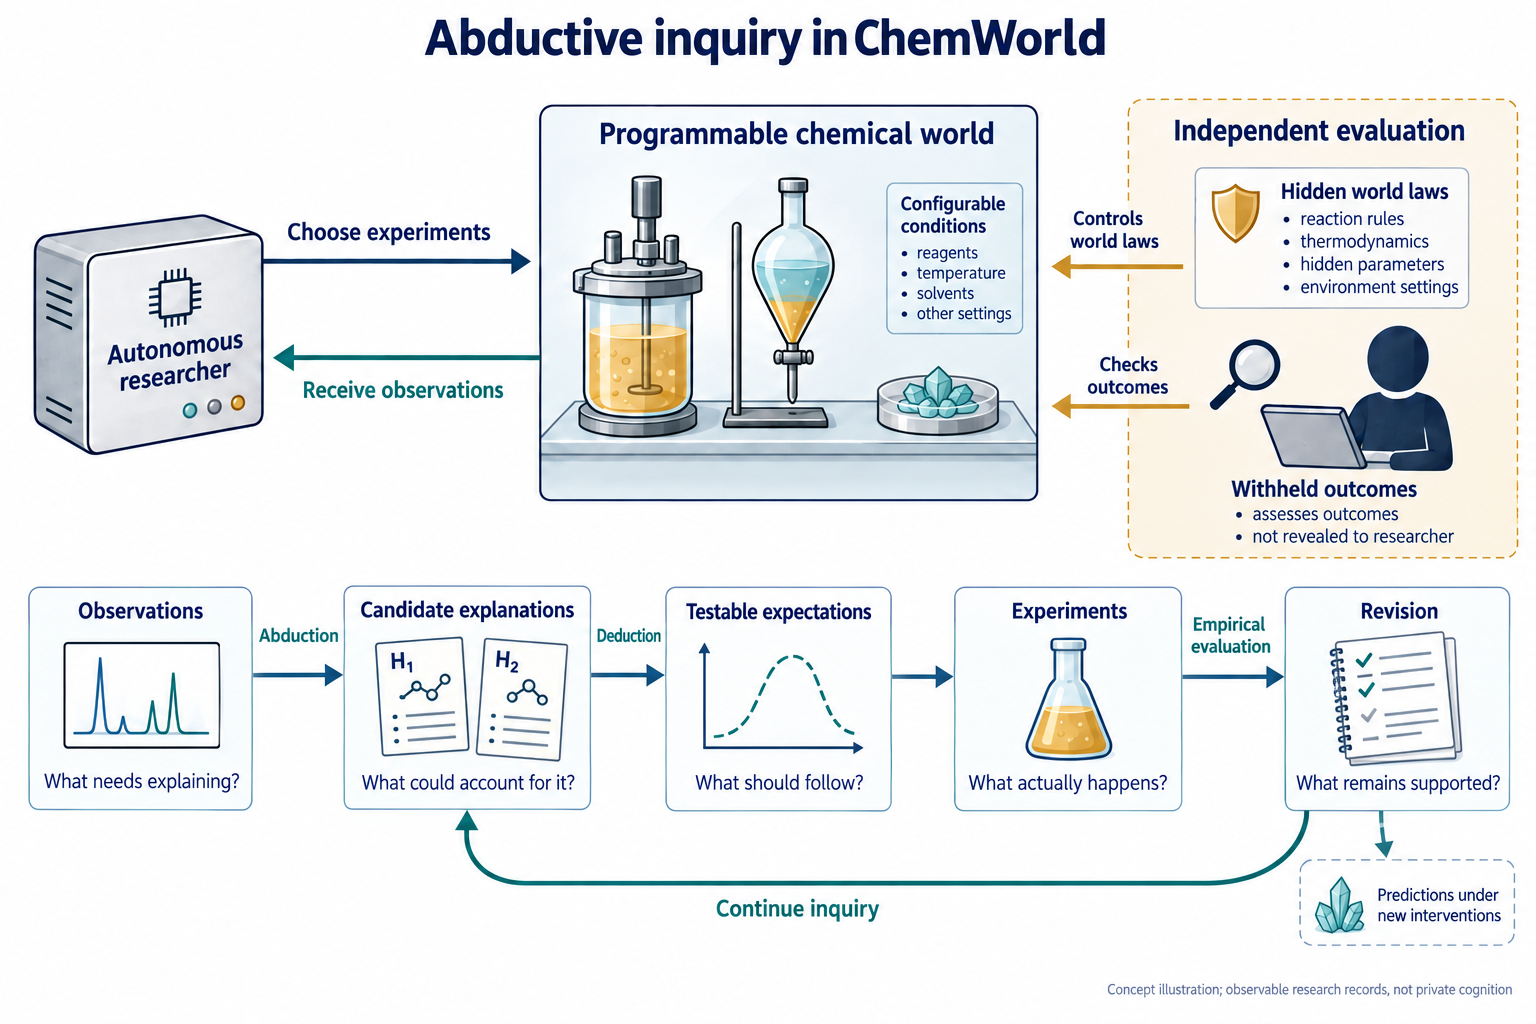
\includegraphics[width=\linewidth,height=.68\textheight,keepaspectratio]{../figures/integrated-20261016/abductive_inquiry.png}}
\caption{Figure 1 \textbar{} Abductive inquiry as an observable research process. ImageGen concept illustration. An autonomous researcher chooses interventions and receives public observations from a persistent chemical world. The evaluator separately controls hidden laws and checks withheld outcomes. The lower cycle distinguishes proposing candidate explanations, deriving testable expectations, performing experiments and revising what remains supported. Revised judgments can guide further inquiry and predictions under new interventions. This is an analytical framework for observable research records, not a claim that every action completes the cycle or a direct measurement of private cognition.}
\end{figure}

\subsection{Research objectives and prior knowledge organize inquiry}\label{research-objectives-and-prior-knowledge-organize-inquiry}

Research starts from goals, available information and a constrained action space. The historical electrochemical and reaction studies ask agents either to develop and test scientific understanding or to optimize a public operating score. These commissions lead to genuine experimental achievements, but operating and predictive gains are not interchangeable (Fig. 2a,b). Optimization produces the better retested electrochemical procedure in 26 of 30 matched comparisons; among those 26, prediction error is lower in thirteen and higher in thirteen. In reaction processing, discovery produces both the better procedure and more accurate score predictions in seventeen of thirty pairs. The relation between a research objective and its scientific consequences therefore depends on what the inquiry actually establishes.

One electrochemical pair makes the distinction concrete (Fig. 2c,d). Discovery compares materials and conditions before increasing duration and current cap; optimization screens material combinations and then refines operating conditions for a promising pair. The optimization recommendation retests at 0.756 against discovery's 0.718, but its prediction mean absolute error (MAE) is 0.229 against 0.088. Its later prediction rationale describes several poorly performing cross-pair combinations as low-activity. That account accompanies a forecast of 0.070 against a reference of 0.494 for one combination under new conditions, while another forecast remains accurate at 0.570 against 0.572. The histories expose what a single endpoint obscures: success in developing a procedure can coexist with uneven judgments about the broader experimental space.

Prior information provides another entry into the organization of inquiry. In corrected crystallization, all fifteen aligned-information sessions start with solvent S2 and catalyst C1, whereas all fifteen sessions without an instance dossier start with S0 and C0. Under the specified mismatched dossier, thirteen start with S2 and fourteen with C1. Mean committed solvent coverage is 2.93, 4.00 and 2.40 for Aligned, Opaque and MisIndexed, respectively. These descriptive differences locate how supplied information enters material selection; wider coverage alone does not establish better learning. In reaction processing, partial parameter knowledge has a clear predictive benefit: Aligned reduces macro MAE from 0.102 to 0.057 under discovery and from 0.139 to 0.084 under optimization, improving on Opaque in four of five worlds under each commission.

\begin{figure}[htbp]
\centering
\pandocbounded{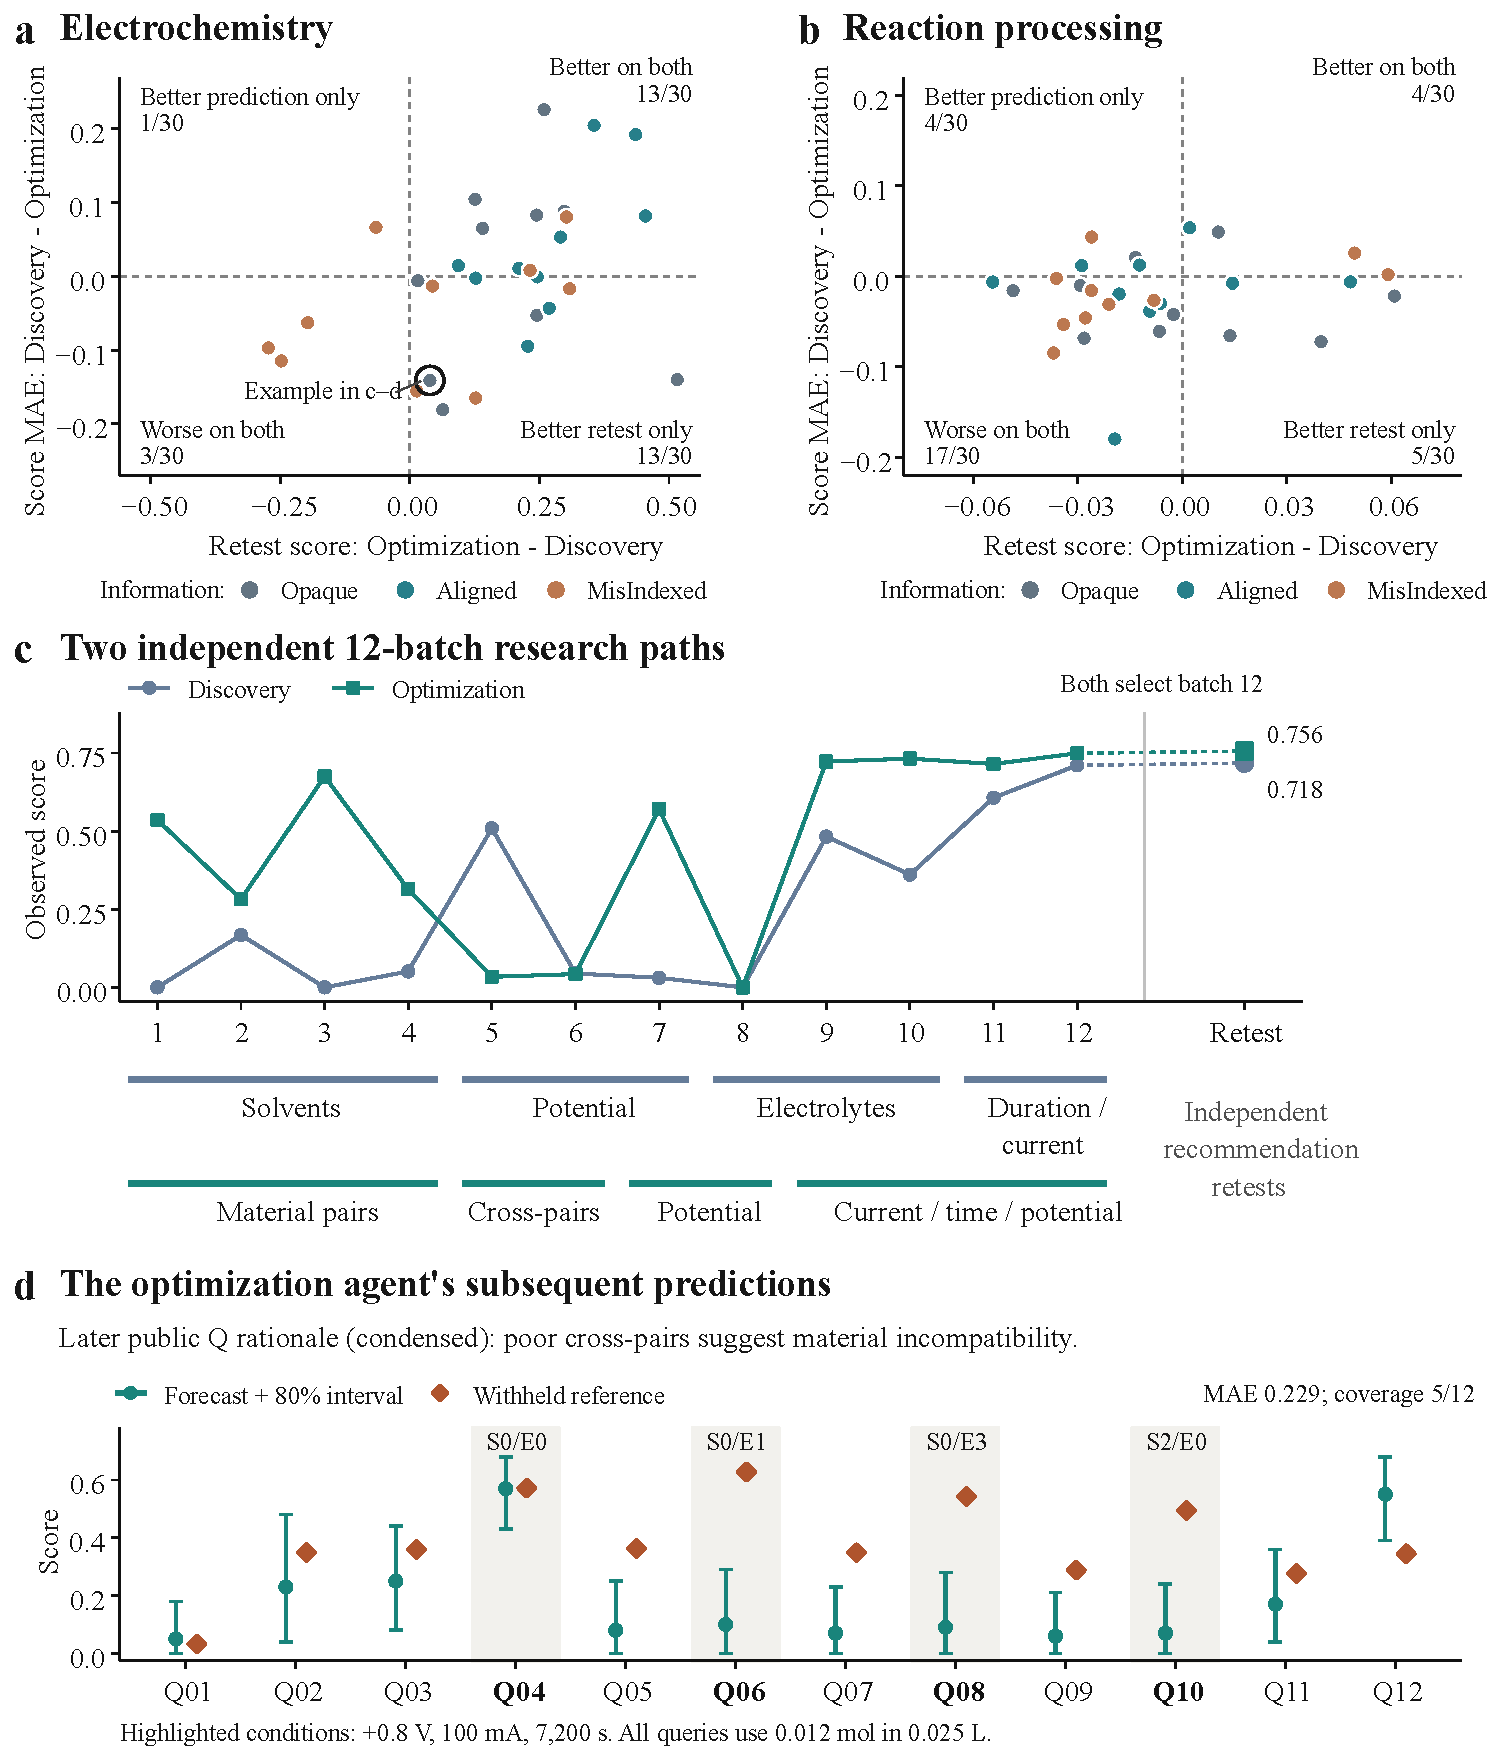
\includegraphics[width=\linewidth,height=.68\textheight,keepaspectratio]{../figures/integrated-20261016/research_objectives.pdf}}
\caption{Figure 2 \textbar{} Experimental achievement and predictive understanding across research objectives. a,b, Thirty matched discovery--optimization pairs in electrochemistry and reaction processing. Positive horizontal values favour optimization on retest score; positive vertical values favour optimization on prediction MAE. Quadrant labels refer to optimization relative to discovery. c, Two independent twelve-batch electrochemical histories and their recommendation retests; batch-phase labels summarize executed choices. d, All twelve optimization forecasts from that pair, with original 80\% intervals and withheld reference outcomes. The later prediction rationale is condensed, not a contemporaneous hypothesis record. The figure retains historical protocols and is not pooled with the repeated process cohort.}
\end{figure}

Research resources likewise support different kinds of progress. Historical independent twelve- and twenty-four-batch campaigns improve some electrochemical, partitioning and crystallization predictions without a corresponding increase in feasible crystallization recommendations or mean retested recovery. These are comparisons of complete resource envelopes, not matched continuations of a single research history. Combined with the goal contrasts in Fig. 2, they show why neither a more productive procedure nor a larger experimental budget alone specifies what scientific relationships have been learned.

\subsection{Explanations develop through conjecture, testing and revision}\label{explanations-develop-through-conjecture-testing-and-revision}

Temporal records allow us to distinguish continuing a predefined scan from revising an explanation in response to an observation. These activities can occupy similar parts of an experimental space. Historical electrochemical discovery and optimization campaigns, for example, cover similar numbers of solvents and both cover all four at the larger budget, despite their differing operating and predictive outcomes. To examine explanatory inquiry, we therefore follow what was expected, what was observed and what the researcher proposed to test next.

A single trajectory from the new opportunity comparison, here called equilibrium study A, makes this transition visible (Fig. 3). Under Opaque information, with no instance-specific archival relationship, the initial note predicts a weak-acid trend: increasing concentration should lower pH and dissociation fraction. The first six experiments instead yield dissociation fractions near 0.064--0.079. The next note withdraws support for the expected trend over the measured range and proposes that a selectable component, rather than the original reagent, might determine the chemically relevant acid loading. It specifies what would support this account: a systematic pH or dissociation response, or a precipitation threshold; flat responses would instead favour a fixed-background or weakly coupled explanation. Batches eight to twelve actually use that component, yet the response remains near a plateau. Its sealed account retains the local relationship and leaves the hidden mechanism unresolved. This connects an initial expectation, discrepant observations, a candidate explanation, discriminating expectations and an executed test within one research history.

This sequence exhibits an observable abductive move: a departure from the initial expectation prompts a new explanatory possibility and an experiment relevant to it. The persistent plateau leaves competing mechanisms unresolved. The evidence therefore establishes an explanatory investigation and a bounded empirical finding, rather than identification of a unique hidden law. This distinction lets the record show scientific progress at the level actually achieved.

Across the corrected crystallization cohort, 52 of 58 selected immediate plans match the ensuing committed actions and six match partly. This measures a public plan--action connection within observable windows, not a discovery rate or an effect of writing the note. Together with the continuous equilibrium case, these records make the adaptation of inquiry observable: an experimental history can enter a revised expectation and a subsequent action. What those actions establish requires examining the content and scope of the resulting relationships.

\begin{figure}[htbp]
\centering
\pandocbounded{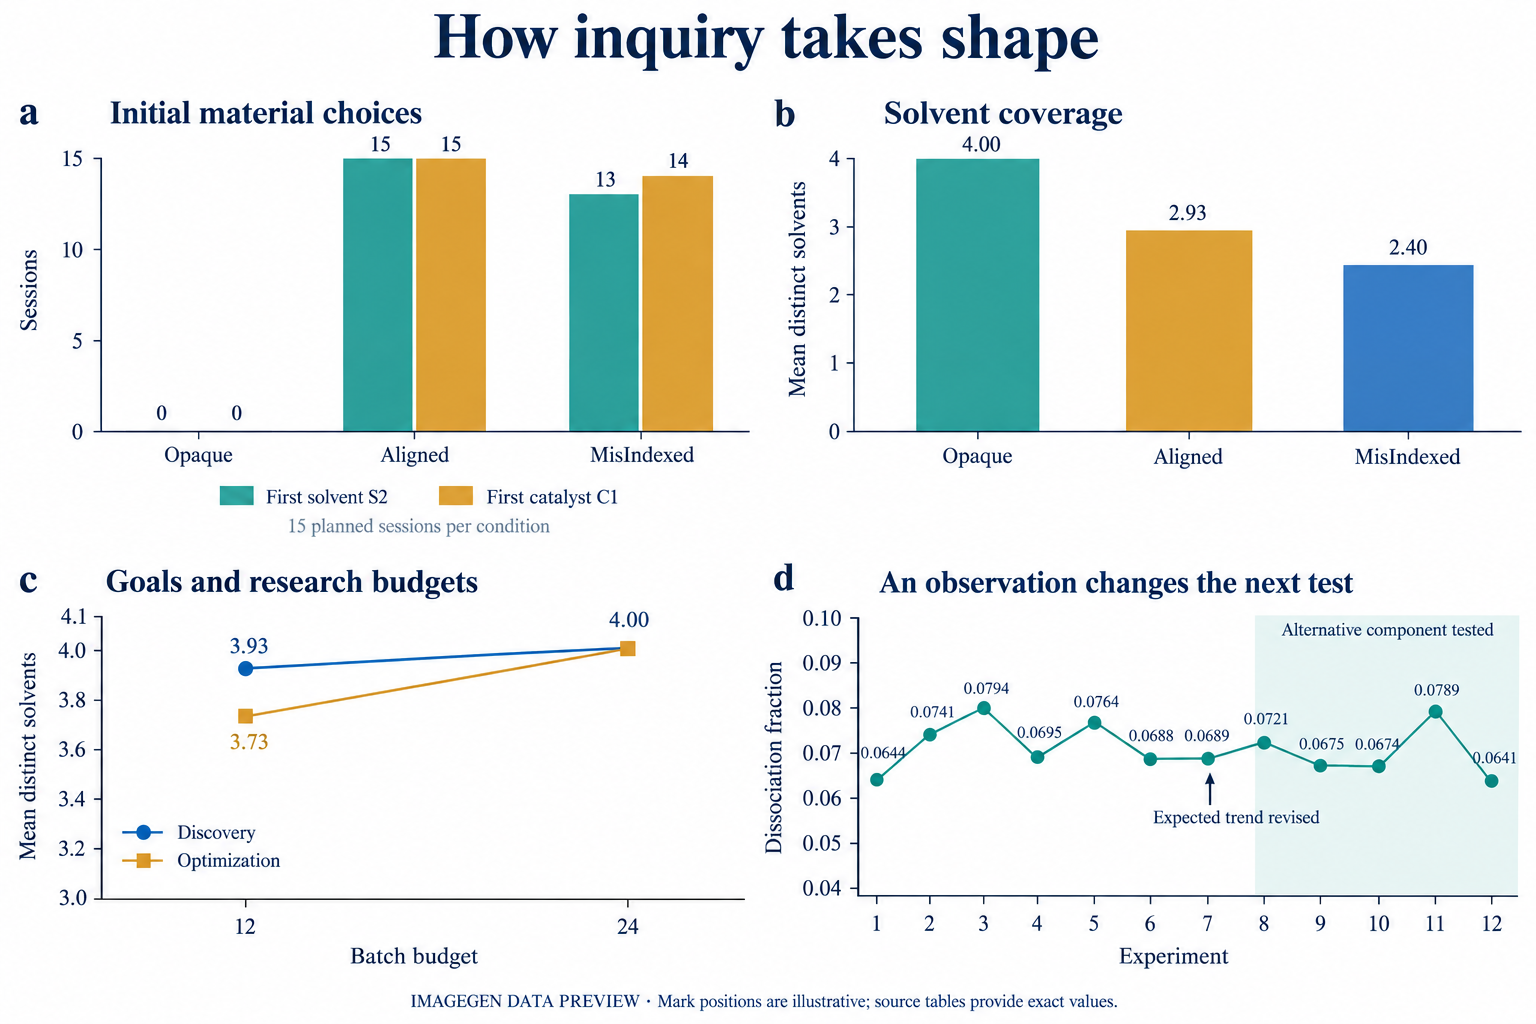
\includegraphics[width=\linewidth,height=.68\textheight,keepaspectratio]{../figures/preview-20261015/figure02.png}}
\caption{Figure 3 \textbar{} Equilibrium study A, from a revised expectation to extrapolation. ImageGen data preview of one continuous Research session and its matched NoResearch forecast. a, The first six assays contradict the expected weak-acid trend within the tested range. b, A new candidate explanation motivates alternative-component tests in batches 8--12; the near-plateau persists. c, The bounded relationship in the sealed account is then given substantial weight in a new dilute prediction; the quotation is verbatim. d, Research predicts dissociation 0.085 {[}0.035, 0.350{]}, NoResearch 0.569 {[}0.040, 0.980{]}, against withheld mean 0.716. Intervals are agent-stated 80\% predictive intervals; source points are individual assays. This is the new opportunity-comparison case, with identity preserved in the evidence archive. Generated geometry is illustrative.}
\end{figure}

Scientific relationships acquire practical meaning when they support a further test, constrain an explanation or guide a new intervention (Fig. 4). In a corrected crystallization study, a near-threshold fines result leads to a prospective proposal to lower the reagent charge from 0.03 to 0.02 mol. The next batch implements that proposal and reduces fines from 0.529 to 0.387, crossing the 0.50 threshold. The result supports a local recipe improvement. Because the absolute catalyst amount remains fixed, however, the catalyst-to-reagent ratio also changes: the experiment does not separately identify a concentration mechanism. What is established is a useful relation between the tested recipes and their outcomes, with a narrower scope than a uniquely identified causal law.

A second crystallization study tests an interpolation. After observing different recovery and fines outcomes at nearby solvent volumes, the researcher proposes that 0.065 L should preserve the recovery benefit while improving fines. The next experiment instead increases fines from 0.512 to 0.601, and the final note retracts the expectation. An unsuccessful operating intervention therefore produces an explicit, evidence-responsive revision. Together with the successful lower-charge test, it shows two ways experimentation can advance a working judgment: establishing a local improvement or withdrawing a prediction the observation does not support.

Whether an intervention actually occurred also determines what can be learned from it. In seed case B, a researcher plans approximately 1 g of cumulative seed addition, but only 0.05 g commits and nineteen subsequent requests are rejected. Its later note correctly recognizes that the high-dose test remains unexecuted. Seed case C encounters analogous rejected requests yet describes 1 g as tested and uses the outcome against a seed-based explanation. These contrasting accounts concern the evidential meaning assigned to the same kind of execution limitation. Additional thermal-history and near-threshold repetition cases remain in the supplementary record.

These episodes expose distinct components of explanatory inquiry. The equilibrium case contains a candidate account of an unexpected response and a test of its consequences; the crystallization cases show prospective expectations, bounded support and revision. Their scientific value lies in what the observations permit the researcher to retain or abandon. A useful intervention, a supported empirical relationship and an identified mechanism are distinguishable achievements, each capable of informing the next investigation.

\begin{figure}[htbp]
\centering
\pandocbounded{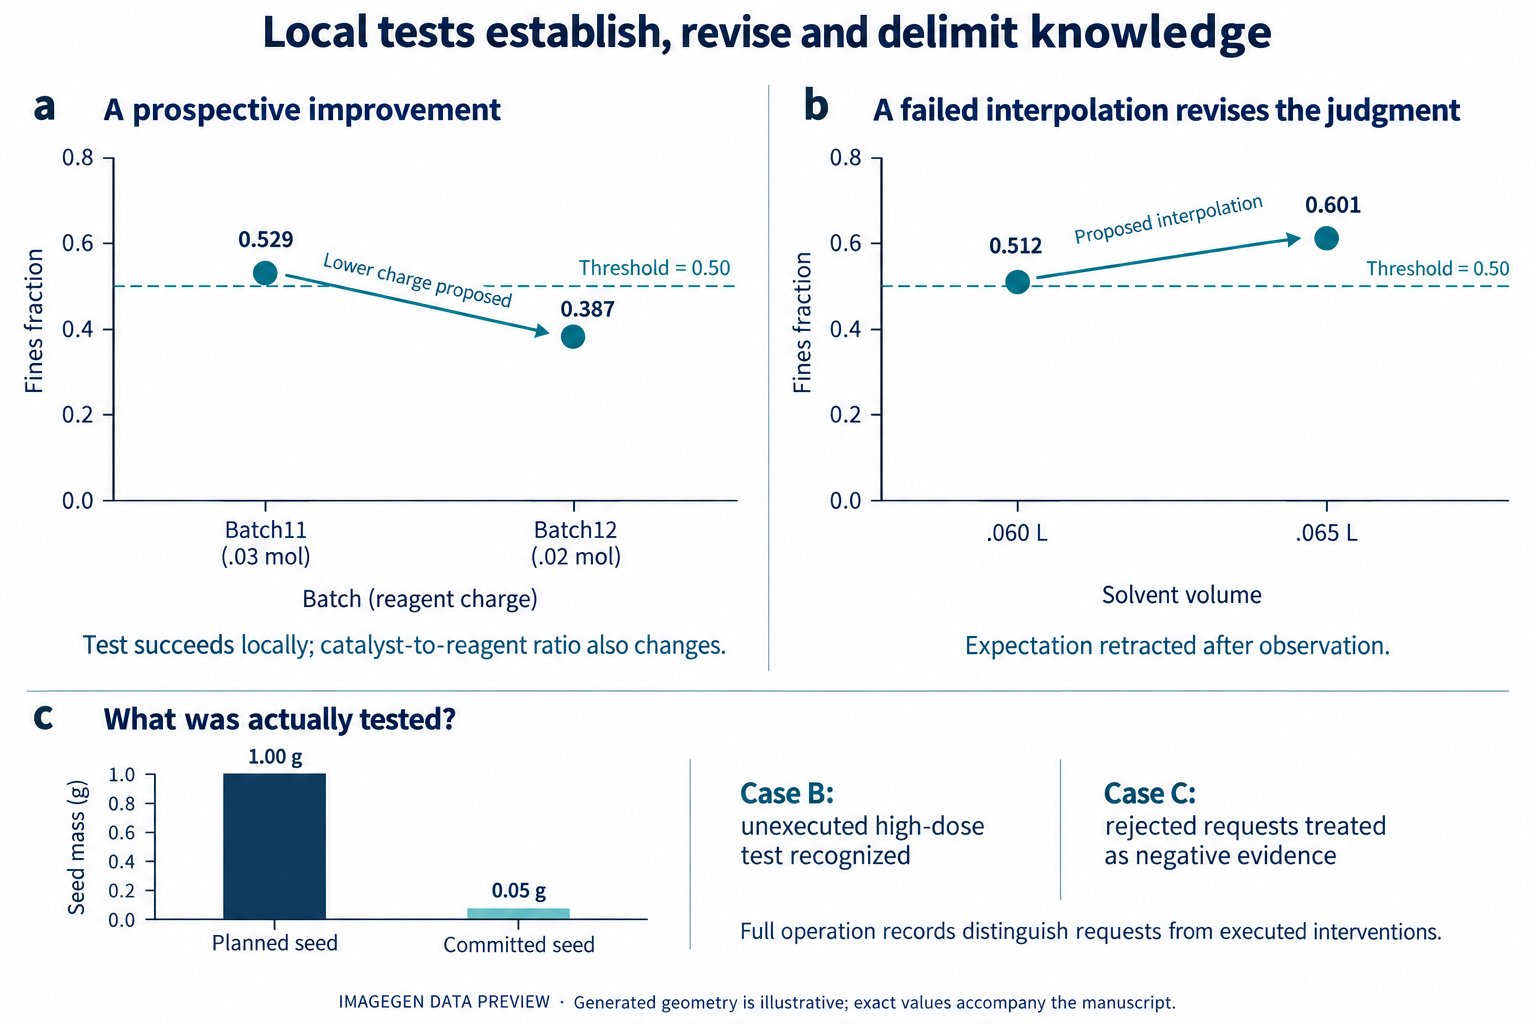
\includegraphics[width=\linewidth,height=.68\textheight,keepaspectratio]{../figures/preview-20261015/figure03.png}}
\caption{Figure 4 \textbar{} Local tests establish, revise and delimit knowledge. ImageGen data preview of distinct crystallization studies. a, Lower charge reduces fines from 0.529 to 0.387, crossing the 0.50 threshold while also changing the catalyst-to-reagent ratio. b, A solvent-volume interpolation raises fines from 0.512 to 0.601; the researcher retracts its expectation. Points in a and b are individual assays, not averages with uncertainty intervals. c, Planned 1 g seed additions leave only 0.05 g committed. Case B recognizes an unexecuted high-dose test; case C treats rejected requests as negative evidence. These are separate researchers, not successive states of one trajectory. Generated geometry is illustrative; complete records accompany the manuscript.}
\end{figure}

\subsection{Different paths from local evidence to extrapolation}\label{different-paths-from-local-evidence-to-extrapolation}

Research paths also differ under the same objective and scientific conditions. In the five-model equilibrium comparison, researchers can choose loading, dilution and addition order before predicting pH, dissociation and precipitation. The hidden laws produce a near-constant dissociation fraction over the higher-concentration region, with a changed response at extreme dilution. Eleven of Astra's fifteen campaigns assay positively loaded samples at nominal concentrations no greater than 1 mM, compared with none of fifteen for each of Sol, GPT-5.5, Luna and Terra (Fig. 5a). This difference describes which evidence these particular campaigns acquire, rather than a fixed exploratory trait of a model.

An Astra campaign illustrates the scientific use of newly acquired evidence (Fig. 5d). Its first three assays show dissociation of 6.3--7.4\%; batch five tests 18.5 micromolar and observes 53.8\%. The later scientific account distinguishes the high-concentration plateau from the dilute response, and the sealed forecast at 13.3 micromolar is 58.80\% with an 80\% interval of 54.20--63.40\%, against a reference mean of 57.97\%. Sol/Opaque takes a different route: despite remaining outside the dilute regime during research, its five-world dilute macro MAE is 0.01833 (Fig. 5b,c). Accurate prediction can therefore accompany either a newly observed change or extrapolation beyond local observations. Direct sampling of every target condition is not a prerequisite for successful inference.

\begin{figure}[htbp]
\centering
\pandocbounded{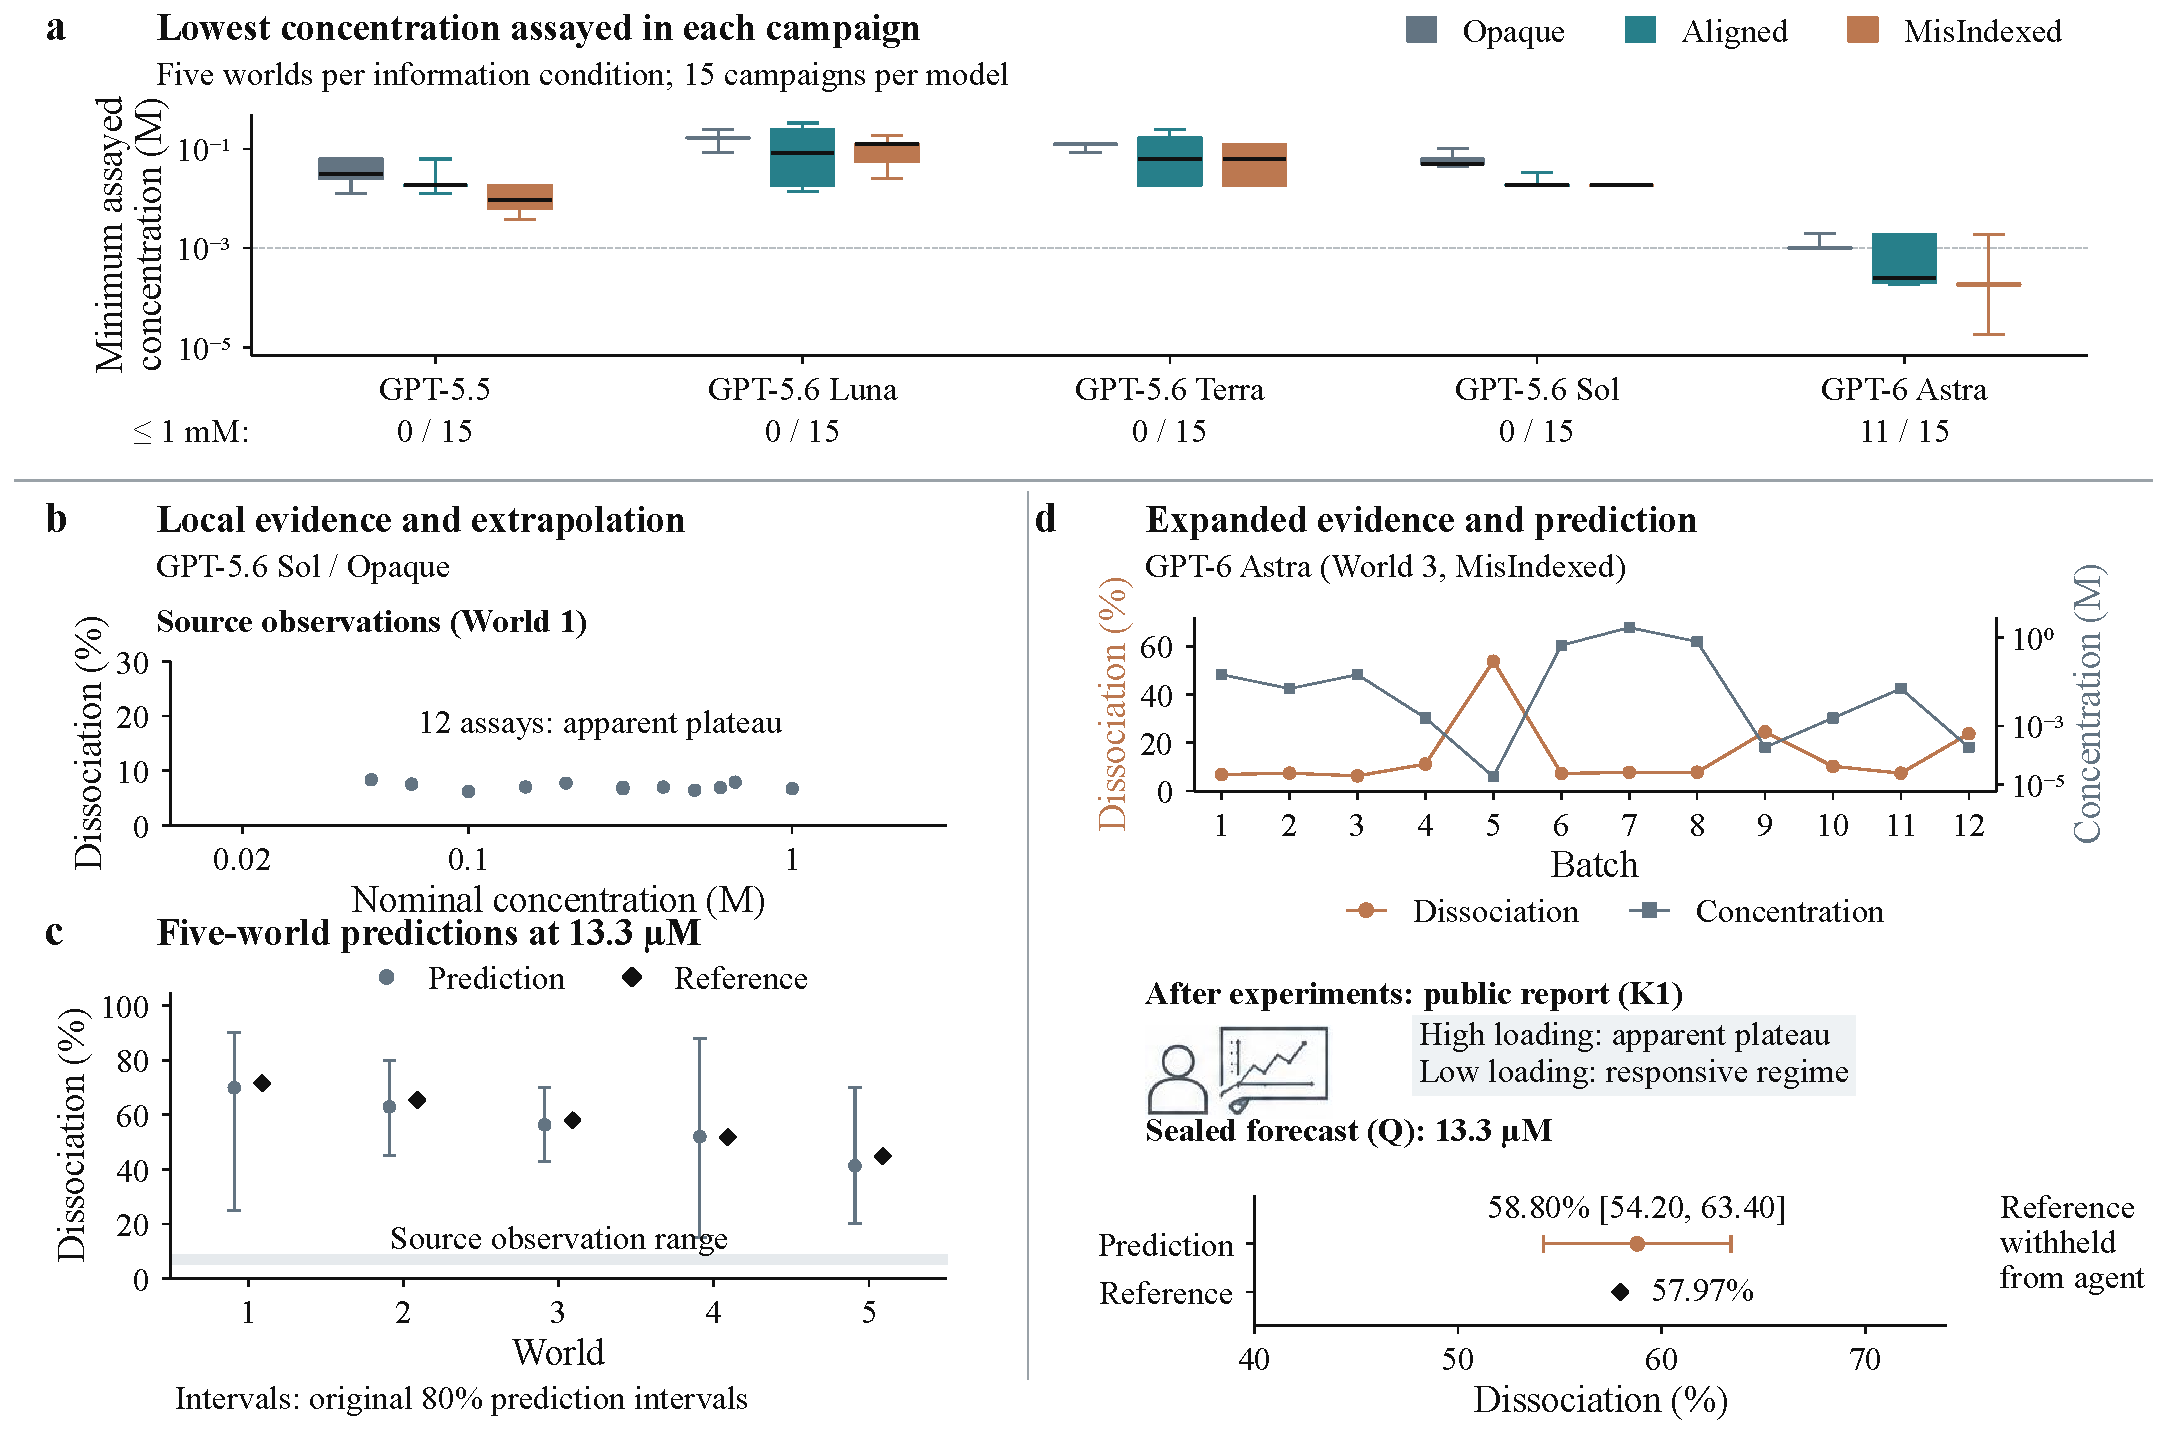
\includegraphics[width=\linewidth,height=.68\textheight,keepaspectratio]{../figures/integrated-20261016/evidence_paths.pdf}}
\caption{Figure 5 \textbar{} Distinct routes from experimental evidence to prediction. a, Minimum positively loaded, assayed concentration for all 75 historical equilibrium campaigns. Each information-arm box contains five world values: median, first and third quartiles, and minimum--maximum whiskers. Quartiles are calculated before logarithmic display. The 1 mM threshold is descriptive. b, Twelve source assays in one Sol/Opaque campaign. c, The most dilute forecast in all five Sol/Opaque worlds, with original 80\% intervals; the shaded band marks source dissociation values. d, All twelve batches of one Astra/MisIndexed campaign, its condensed post-experiment account and a sealed forecast. The account is retrospective, not a quotation of contemporaneous reasoning. These data distinguish expanded evidence acquisition from extrapolation beyond local evidence, without assigning either route a model-wide cognitive mechanism.}
\end{figure}

The crucial question is what these different routes establish. Extrapolation can be scientifically legitimate without direct measurement of every target condition, but its support depends on the available theory, observations and unresolved alternatives. Following a judgment from its local evidential basis into a new use exposes that distinction.

The same equilibrium study A now connects a warranted local revision to its later use (Fig. 3c,d). When forecasting an extremely dilute condition, the agent writes: ``The point estimate still favors the experimentally supported fixed acidic background''. It predicts dissociation of 0.085 with an 80\% interval of 0.035--0.350; the withheld reference mean is 0.716. Both its scientific account and forecast recognize that this regime was not tested. The transition is therefore more specific than an omitted caveat: a relationship supported locally receives substantial weight in a prediction whose continuation the experiments have not resolved. The matched no-research forecast for the same query is 0.569, with interval 0.040--0.980, and explicitly relies on an untested prior assumption. Its greater numerical accuracy does not establish a better experimental discovery.

That continuation is not inevitable. Two sessions in another fixed equilibrium world both observe plateaux at relatively high loading, yet their dilute macro errors are 0.16287 and 0.01462. For the same dilute query, they predict dissociation of 0.130 and 0.626 against a reference mean of 0.65463. The more accurate session uses a weak-acid continuation consistent with its plateau observations and explicitly describes it as conjectural. Together with the historical Sol/Opaque and Astra cases, these records distinguish several routes to a judgment: an observed change, a plausible extrapolation and a local relationship carried into an unresolved regime. Numerical correctness and experimental establishment remain separate questions.

The equilibrium prior comparison contrasts with the positive reaction results. In the original Sol campaigns, correct partial information lowers macro MAE on nine queries from 0.01008 to 0.00465, yet increases it on the three most dilute queries from 0.01833 to 0.15862. Both directions occur in all five worlds. A separate repeated cohort shows the same aggregate directions with different magnitudes: 0.00907 to 0.00512 on nine queries and 0.09880 to 0.13205 on the dilute subset. These cohorts are reported separately. The model comparison further limits the interpretation (Fig. 6c): Luna and Terra improve with Aligned information in both regions, GPT-5.5 changes little, and Astra retains low dilute error across all three arms. The effect of partial knowledge is therefore conditional on both the researcher and the condition being judged; a local benefit does not determine its value elsewhere.

\begin{figure}[htbp]
\centering
\pandocbounded{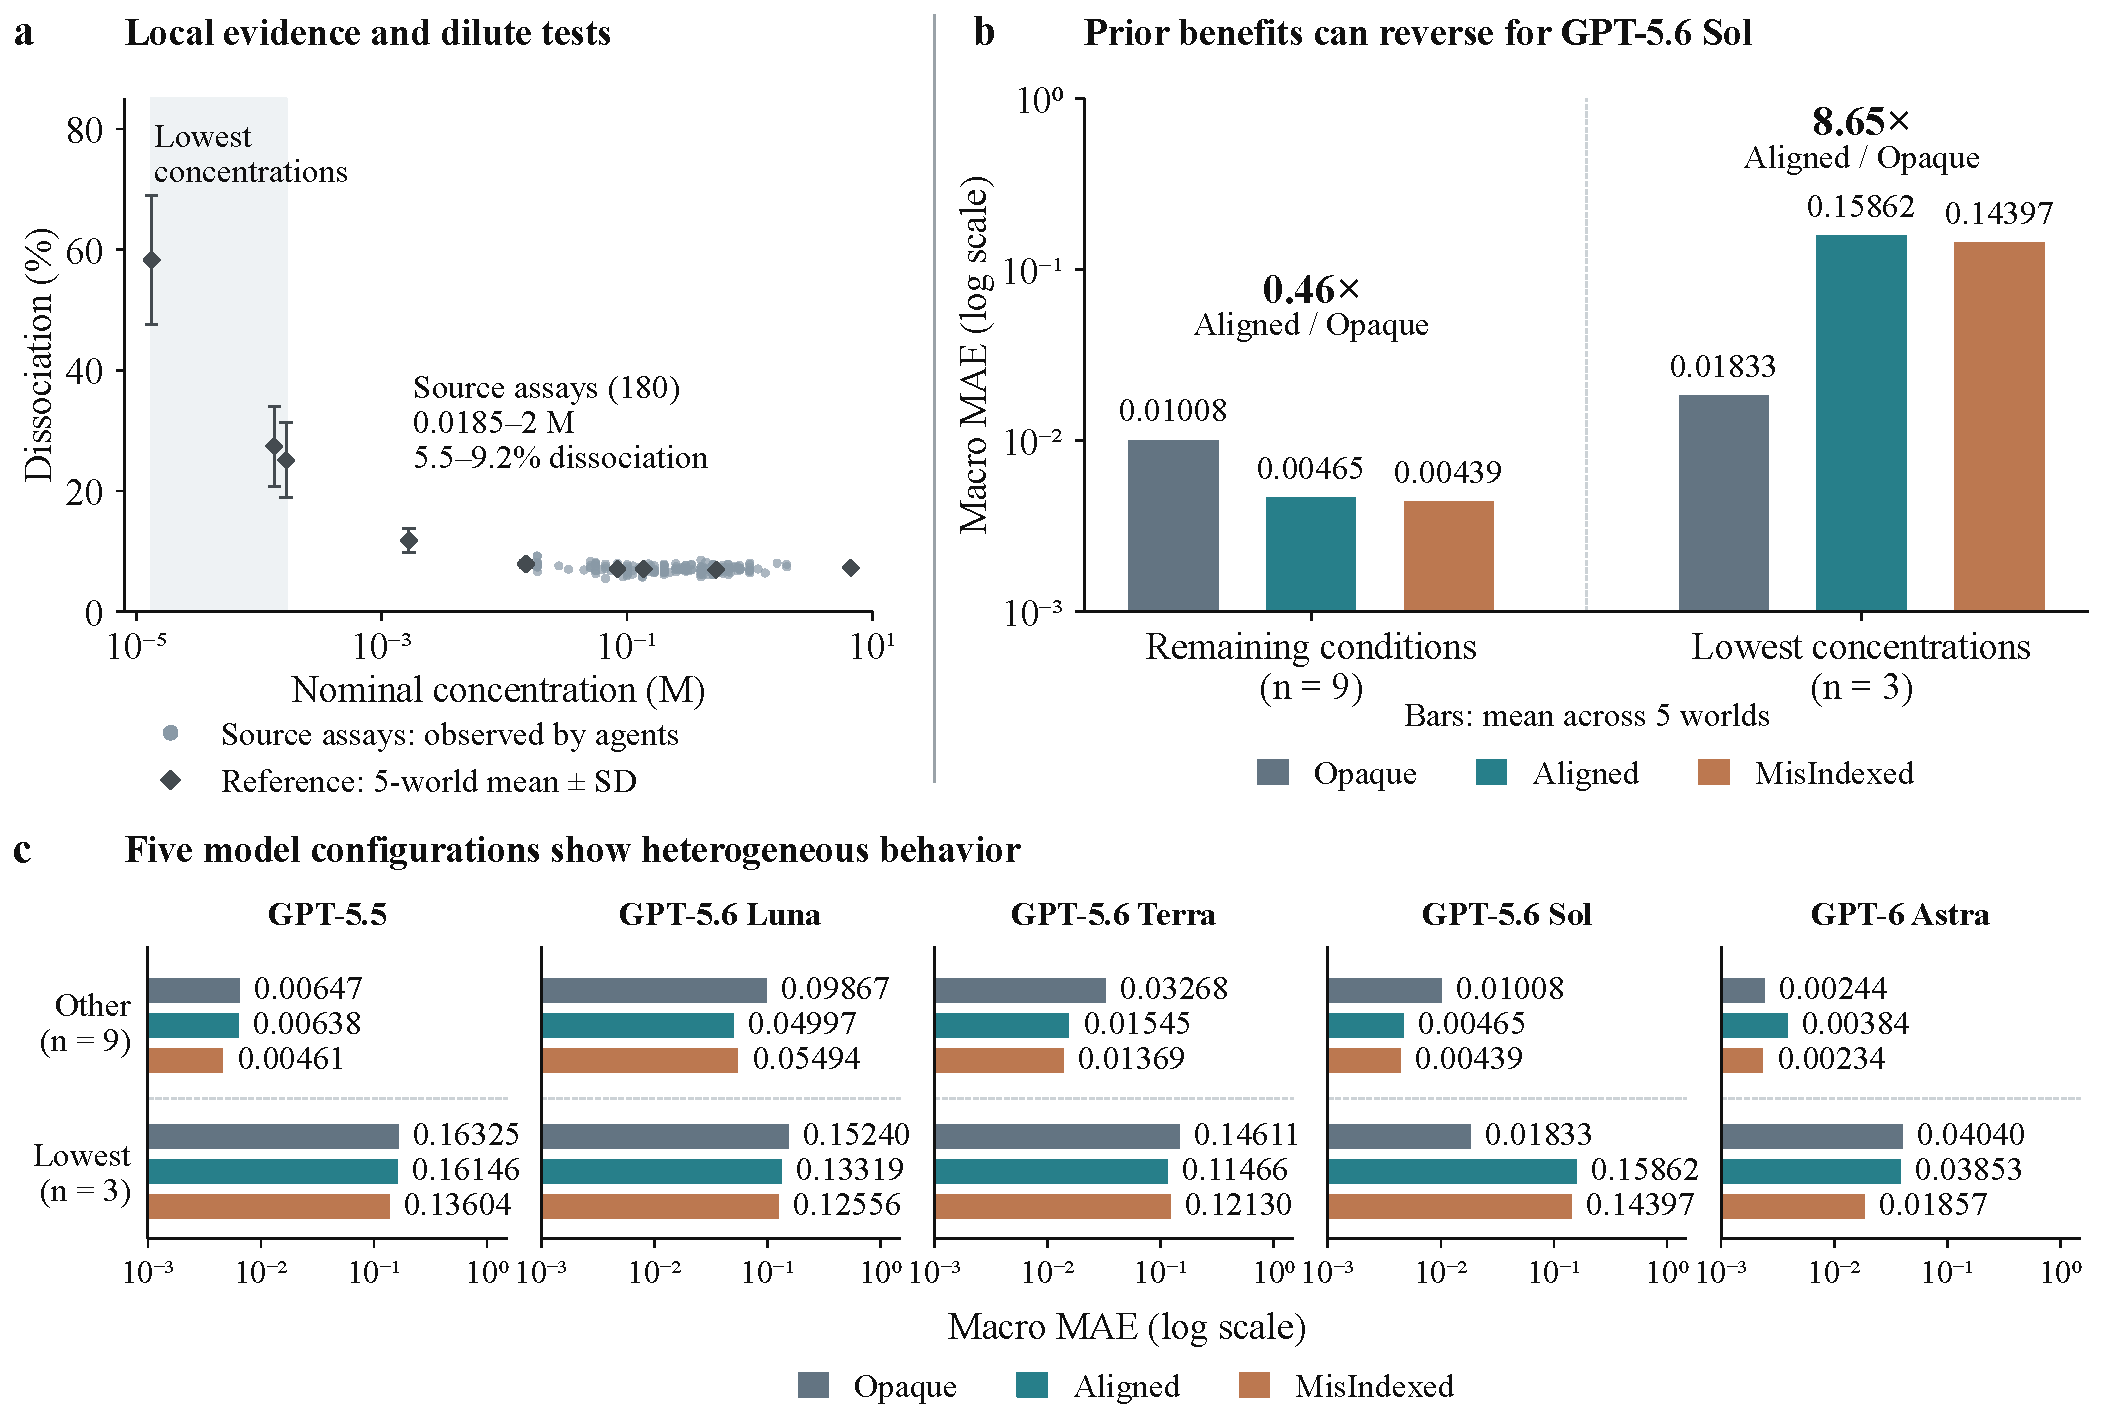
\includegraphics[width=\linewidth,height=.68\textheight,keepaspectratio]{../figures/integrated-20261016/priors_and_transfer.pdf}}
\caption{Figure 6 \textbar{} The reach of partial prior knowledge depends on the researcher and the condition. Original equilibrium comparison. a, All 180 Sol source assays and withheld query means across five worlds; error bars are descriptive sample SD, not confidence intervals. b, Five-world macro MAE for Sol under three information conditions. c, All five model configurations on the same logarithmic error scale. Bar baselines are 0.001. The three lowest-concentration queries and remaining nine were a post hoc partition of this historical cohort, fixed before subsequent repeated blocks. These are historical results; the separate repeated-cohort values in the text are not added to these bars. Each model--world--information cell contains one campaign.}
\end{figure}

\subsection{Research changes the reach of scientific understanding}\label{research-changes-the-reach-of-scientific-understanding}

Explanations must remain useful as research moves beyond the conditions under which they formed. We therefore complement the observed inference paths with a controlled comparison of research opportunity, followed by response-specific checks on how acquired evidence enters new predictions.

The matched research-opportunity comparison asks a more direct question: does access to research change subsequent prediction under common initial scientific information (Fig. 7)? All thirty sessions use Opaque information: the public task, material identities, measurement scales, legal operations and initial state are available, but no instance-specific archival law or fitted relationship is supplied. Each of five equilibrium worlds receives three fresh sessions with twelve source batches and three without source experiments. Scientific inputs and sealed assessments are matched within each world and repeat. All thirty sessions terminate, all 180 planned source batches complete, and twenty-nine sessions provide valid forecasts. One research session loses its forecast and later stages to a network interruption; its observations and scientific account remain retained.

\begin{figure}[htbp]
\centering
\pandocbounded{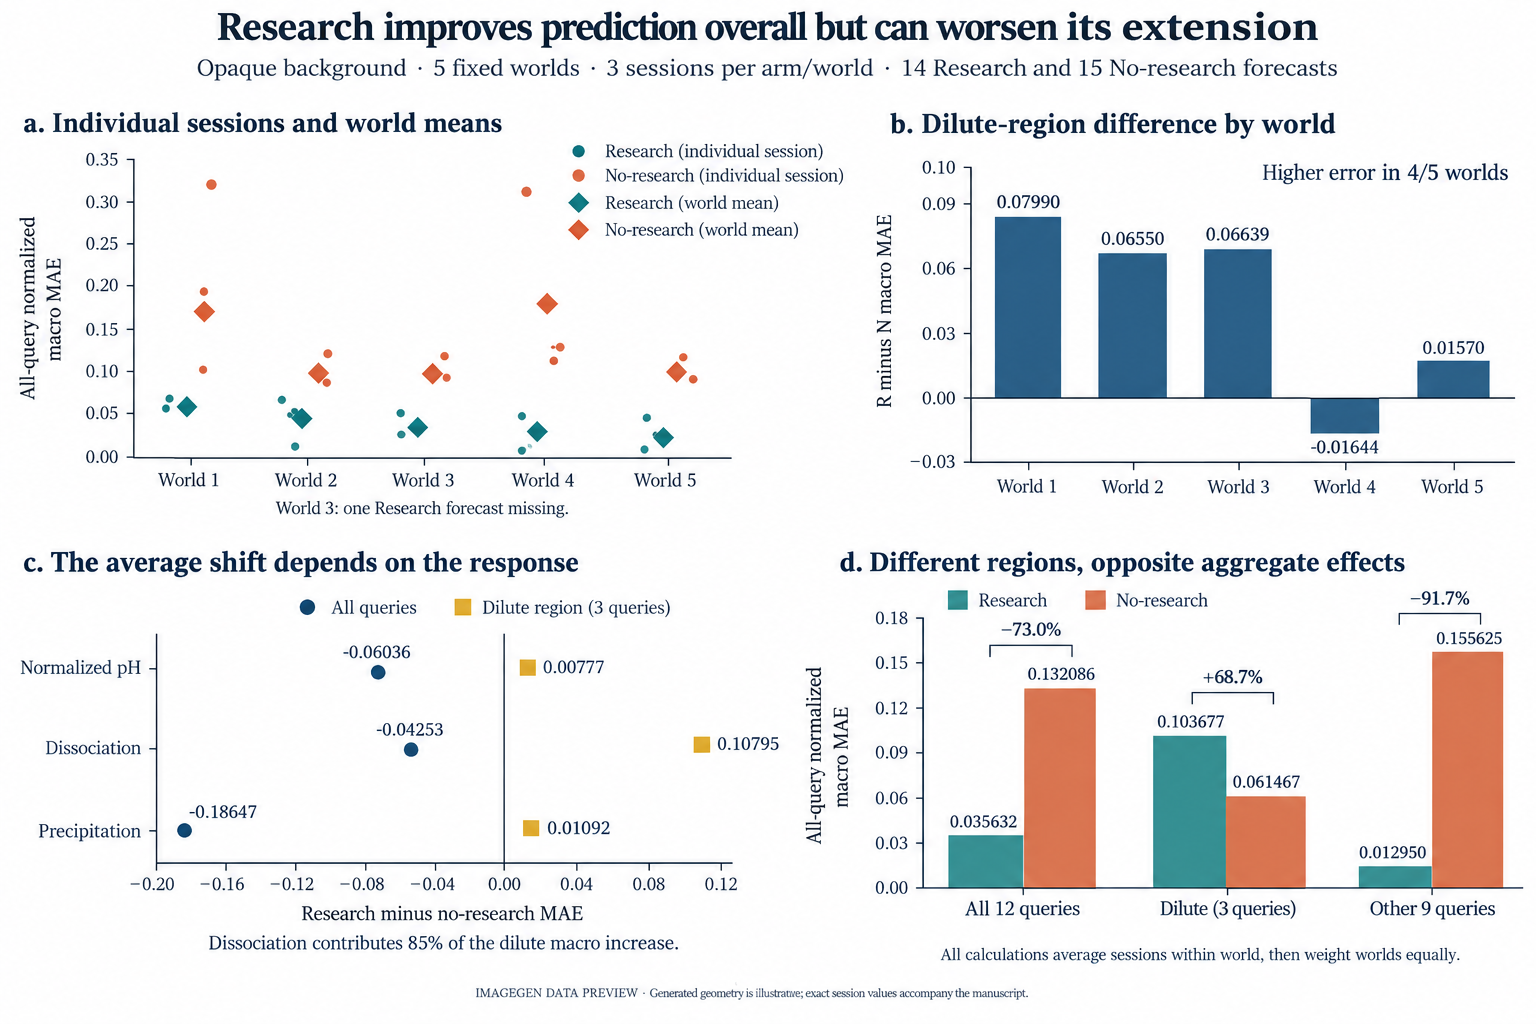
\includegraphics[width=\linewidth,height=.68\textheight,keepaspectratio]{../figures/preview-20261015/figure04.png}}
\caption{Figure 7 \textbar{} Overall gains and a regional reversal from research. ImageGen data preview. All thirty sessions use Opaque information and matched scientific inputs. a, Individual all-query macro errors and within-world means; Research has fourteen valid forecasts and NoResearch fifteen. World 3 has one retained missing Research forecast. b, Dilute-region Research-minus-NoResearch macro error is positive in four of five worlds. c, Response-specific shifts differ; dissociation contributes 85.2\% of the dilute macro increase. d, Equal-world errors across all twelve, dilute three and other nine queries change by −73.0\%, +68.7\% and −91.7\%, respectively. Generated dots and geometry are illustrative; exact session values, response errors and all 1,044 valid query-response rows are supplied in the evidence archive. No confidence intervals or population sampling inference are implied.}
\end{figure}

Research substantially improves prediction overall. Averaging valid sessions within each world and then weighting the five worlds equally, normalized macro mean absolute error falls from 0.132086 without research to 0.035632 with research, a 73.0\% reduction. The direction holds in all five worlds. Yet for the three prospectively designated extreme-dilution queries, error rises from 0.061467 to 0.103677, a 68.7\% increase, with deterioration in four of five worlds. Over the remaining nine queries it falls from 0.155625 to 0.012950. The comparison concerns the total opportunity to conduct research, including experiment selection, feedback and available recording tools; it does not isolate any one component.

Within this comparison, the same research opportunity improves overall prediction while worsening it in a defined region. All three response-specific point errors increase on the dilute subset, but by different amounts: Research-minus-NoResearch MAE is +0.00777 for normalized pH, +0.10795 for dissociation fraction and +0.01092 for precipitation signal. Dissociation accounts for 85.2\% of the macro-error increase. Figure 7 shows individual sessions and world means; the complete session-by-response and query-level results accompany the manuscript. Equilibrium study A supplies one observed route from a valid local finding to a distant judgment. It does not establish that this route explains every session-level difference or that acquiring more evidence must impair extrapolation.

The result extends beyond point error without yielding a universal story of misplaced confidence. At extreme dilution, research produces lower empirical coverage than no research for all three nominal 80\% intervals, while the no-research intervals are substantially wider. An interval score penalizing both width and misses favours research for pH, favours no research for dissociation fraction and is similar for precipitation signal. Across all queries, research improves interval scores for all three responses. A conservative sensitivity analysis allowing the missing session's macro error to take any value in its legal range does not reverse either the overall benefit or the dilute deterioration (Methods).

Crystallization exposes a complementary pattern in the use of evidence already acquired (Extended Data Fig. 2). For each of 42 valid forecasts, transparent references use only that same session's source observations. Five-world-equal purity error is 0.03853 for the agent and 0.00510 for the overall source mean, which is more accurate in every valid session. Recovery shows the opposite pattern: agent error is 0.10129 against 0.20443, with the agent outperforming the mean in 39 of 42 sessions. Conditioning on the exact committed solvent set preserves both aggregate directions. Size and fines yield 5/42 and 23/42 wins, respectively. These references diagnose how acquired evidence is used across responses; they are neither no-research controls nor alternative autonomous researchers, and do not estimate the causal benefit of crystallization research.

This response-specific comparison complements the equilibrium result. The challenge is not only to anticipate change beyond an observed region, but also to preserve a relationship when it remains useful. Within the same crystallization histories, predictions extract information about varying recovery more effectively than the source mean, yet fail to match that simple reference for stable purity. Successful evidence use in one response does not establish that all acquired relationships constrain subsequent judgments equally. Across objectives, priors, budgets and research access, scientific progress therefore has several observable dimensions: what is achieved experimentally, what the evidence establishes and how well the resulting relationships guide new judgments.

\FloatBarrier
\subsection{Discussion}\label{discussion}

Abductive inquiry gives autonomous science a substantive object of evaluation: the development of explanations through research. The present studies connect the conditions under which agents investigate, the hypotheses and relationships they express, the tests they execute and the judgments they subsequently make. Cross-system comparisons establish that operating success and predictive understanding can develop differently. Contemporaneous cases show that this divergence can coexist with meaningful scientific activity, including proposing an alternative explanation, testing a local expectation and retracting it when the observation disagrees. The unit of analysis is the explanation in its research history, with the evidence and uses that give it scientific significance.

The results distinguish proposing an explanation, supporting it experimentally and applying it successfully. In equilibrium study A, a plausible candidate motivates an executed test without uniquely identifying the hidden mechanism. In crystallization, a successful recipe change establishes a useful intervention while leaving correlated causes unresolved; a failed interpolation supports a warranted retraction. The Astra and Sol/Opaque histories further show that accurate predictions can follow direct observation of a changed response or a conjectural continuation beyond local evidence. These are different scientific achievements. Their distinction is lost when all experiments are treated as interchangeable data collection or all correct predictions as equivalent evidence of discovery.

This perspective places abduction within a continuing interaction with deduction and empirical testing. A candidate explanation opens a possible account of observations; its consequences guide tests; their outcomes can strengthen, delimit or displace it. The empirical records also show where this relationship becomes incomplete: a rejected operation can be remembered as a completed test, a local regularity can dominate an unresolved extrapolation, or an established response can fail to constrain prediction. Discovery and misunderstanding can therefore arise at different points within the same inquiry. Examining those transitions makes it possible to ask what a researcher has reason to conclude, as well as whether its conclusion happens to be correct\textsuperscript{12,22,23}.

The controlled comparisons complement this process account. Research goals, prior information and available resources reveal different conditions of inquiry; the matched opportunity study examines the total contribution of conducting research under common initial information. Its overall gains and regional reversal show that scientific benefit can depend on the question being asked. They do not isolate an effect of abduction, autonomy, feedback or notebook use. A separate fixed-recipe quench comparison identifies physical consequences of an intervention without providing feedback to an adapting agent (Extended Data Fig. 3). Temporal links between public judgments and actions likewise do not establish a unique causal mechanism for their formation. These distinctions allow different experiments to contribute to a common question without assigning them the same causal claim.

The study concerns selected programmable systems and a small fixed set of worlds; repeated process analysis uses one model configuration. Fresh sessions are not controlled model-seed replications or independent samples of world laws. Public notes do not expose private cognition, and observable explanatory activity does not establish the invention of a novel scientific theory. The framework organizes interpretation of retained evidence rather than a new quantitative test of abductive ability. Cases are retrospectively selected, with single-analyst interpretation and no second-rater reliability estimate. Historical and current protocols retain separate provenance, including corrected crystallization and all failures. These boundaries specify the scale at which the observed formation, testing and use of explanations are supported.

The broader ambition is to understand how a system capable of experimenting can become a system capable of developing scientific explanations. Einstein's example motivates the intellectual demand, while programmable worlds make particular components of that demand accessible to controlled study. ChemWorld connects the explanations an agent proposes to the experiments it chooses and to the evidence that can change its account of the world. Scientific autonomy develops through this continuing responsiveness: the ability to pursue an explanation, determine what it establishes and revise its reach as inquiry proceeds.

\subsection{Funding}\label{funding}

This work was supported by the Shenzhen Science and Technology Program (AI2026004), the Tsinghua University Initiative Scientific Research Program and the Scientific Research Innovation Capability Support Project for Young Faculty (ZYGXQNJSKYCXNLZCXM-E7).

\clearpage
\onecolumn

\section{References}\label{references}

\protect\phantomsection\label{refs}
\begin{CSLReferences}{0}{1}
\hypertarget{ref-einstein1905electrodynamics}{}
\CSLLeftMargin{1. }%
\CSLRightInline{A. Einstein. Zur elektrodynamik bewegter k{ö}rper. \emph{Annalen der Physik} \textbf{322} 891--921 (1905). https://doi.org/\href{https://doi.org/10.1002/andp.19053221004}{10.1002/andp.19053221004}.}

\hypertarget{ref-douven2025peirce}{}
\CSLLeftMargin{2. }%
\CSLRightInline{I. Douven. Peirce on abduction. \emph{The stanford encyclopedia of philosophy: abduction} (2025). \url{https://plato.stanford.edu/entries/abduction/peirce.html}.}

\hypertarget{ref-tom2024selfdriving}{}
\CSLLeftMargin{3. }%
\CSLRightInline{G. Tom et al. {Self-Driving Laboratories for Chemistry and Materials Science}. \emph{Chemical Reviews} \textbf{124} 9633--9732 (2024). https://doi.org/\href{https://doi.org/10.1021/acs.chemrev.4c00055}{10.1021/acs.chemrev.4c00055}.}

\hypertarget{ref-boiko2023autonomous}{}
\CSLLeftMargin{4. }%
\CSLRightInline{D. A. Boiko, R. MacKnight, B. Kline, and G. Gomes. Autonomous chemical research with large language models. \emph{Nature} \textbf{624} 570--578 (2023). https://doi.org/\href{https://doi.org/10.1038/s41586-023-06792-0}{10.1038/s41586-023-06792-0}.}

\hypertarget{ref-king2009automation}{}
\CSLLeftMargin{5. }%
\CSLRightInline{R. D. King et al. {The Automation of Science}. \emph{Science} \textbf{324} 85--89 (2009). https://doi.org/\href{https://doi.org/10.1126/science.1165620}{10.1126/science.1165620}.}

\hypertarget{ref-burger2020mobile}{}
\CSLLeftMargin{6. }%
\CSLRightInline{B. Burger et al. {A mobile robotic chemist}. \emph{Nature} \textbf{583} 237--241 (2020). https://doi.org/\href{https://doi.org/10.1038/s41586-020-2442-2}{10.1038/s41586-020-2442-2}.}

\hypertarget{ref-macleod2020selfdriving}{}
\CSLLeftMargin{7. }%
\CSLRightInline{B. P. MacLeod et al. {Self-driving laboratory for accelerated discovery of thin-film materials}. \emph{Science Advances} \textbf{6} eaaz8867 (2020). https://doi.org/\href{https://doi.org/10.1126/sciadv.aaz8867}{10.1126/sciadv.aaz8867}.}

\hypertarget{ref-szymanski2023alab}{}
\CSLLeftMargin{8. }%
\CSLRightInline{{N. J. Szymanski et al.} An autonomous laboratory for the accelerated synthesis of inorganic materials. \emph{Nature} \textbf{624} 86--91 (2023). https://doi.org/\href{https://doi.org/10.1038/s41586-023-06734-w}{10.1038/s41586-023-06734-w}.}

\hypertarget{ref-bran2024augmenting}{}
\CSLLeftMargin{9. }%
\CSLRightInline{A. M. Bran et al. Augmenting large language models with chemistry tools. \emph{Nature Machine Intelligence} \textbf{6} 525--535 (2024). https://doi.org/\href{https://doi.org/10.1038/s42256-024-00832-8}{10.1038/s42256-024-00832-8}.}

\hypertarget{ref-dai2024mobile}{}
\CSLLeftMargin{10. }%
\CSLRightInline{T. Dai et al. {Autonomous mobile robots for exploratory synthetic chemistry}. \emph{Nature} \textbf{635} 890--897 (2024). https://doi.org/\href{https://doi.org/10.1038/s41586-024-08173-7}{10.1038/s41586-024-08173-7}.}

\hypertarget{ref-elmachtoub2022spo}{}
\CSLLeftMargin{11. }%
\CSLRightInline{A. N. Elmachtoub and P. Grigas. Smart {Predict, then Optimize}. \emph{Management Science} \textbf{68} 9--26 (2022). https://doi.org/\href{https://doi.org/10.1287/mnsc.2020.3922}{10.1287/mnsc.2020.3922}.}

\hypertarget{ref-shmueli2010explain}{}
\CSLLeftMargin{12. }%
\CSLRightInline{G. Shmueli. {To Explain or to Predict?} \emph{Statistical Science} \textbf{25} 289--310 (2010). https://doi.org/\href{https://doi.org/10.1214/10-sts330}{10.1214/10-sts330}.}

\hypertarget{ref-platt1964inference}{}
\CSLLeftMargin{13. }%
\CSLRightInline{J. R. Platt. {Strong Inference}. \emph{Science} \textbf{146} 347--353 (1964). https://doi.org/\href{https://doi.org/10.1126/science.146.3642.347}{10.1126/science.146.3642.347}.}

\hypertarget{ref-lindley1956information}{}
\CSLLeftMargin{14. }%
\CSLRightInline{D. V. Lindley. {On a Measure of the Information Provided by an Experiment}. \emph{The Annals of Mathematical Statistics} \textbf{27} 986--1005 (1956). https://doi.org/\href{https://doi.org/10.1214/aoms/1177728069}{10.1214/aoms/1177728069}.}

\hypertarget{ref-chaloner1995design}{}
\CSLLeftMargin{15. }%
\CSLRightInline{K. Chaloner and I. Verdinelli. {Bayesian Experimental Design: A Review}. \emph{Statistical Science} \textbf{10} 273--304 (1995). https://doi.org/\href{https://doi.org/10.1214/ss/1177009939}{10.1214/ss/1177009939}.}

\hypertarget{ref-mirza2025chembench}{}
\CSLLeftMargin{16. }%
\CSLRightInline{A. Mirza et al. {A framework for evaluating the chemical knowledge and reasoning abilities of large language models against the expertise of chemists}. \emph{Nature Chemistry} \textbf{17} 1027--1034 (2025). https://doi.org/\href{https://doi.org/10.1038/s41557-025-01815-x}{10.1038/s41557-025-01815-x}.}

\hypertarget{ref-majumder2025discoverybench}{}
\CSLLeftMargin{17. }%
\CSLRightInline{B. P. Majumder et al. {DiscoveryBench: Towards Data-Driven Discovery with Large Language Models}. \emph{{International Conference on Learning Representations}} \textbf{2025} 4556--4579 (2025). \url{https://proceedings.iclr.cc/paper_files/paper/2025/file/0d70af566e69f1dfb687791ecf955e28-Paper-Conference.pdf}.}

\hypertarget{ref-wang2022scienceworld}{}
\CSLLeftMargin{18. }%
\CSLRightInline{R. Wang, P. Jansen, M.-A. Côté, and P. Ammanabrolu. {ScienceWorld: Is your Agent Smarter than a 5th Grader?} \emph{Proceedings of the 2022 conference on empirical methods in natural language processing} 11279--11298 (2022). https://doi.org/\href{https://doi.org/10.18653/v1/2022.emnlp-main.775}{10.18653/v1/2022.emnlp-main.775}.}

\hypertarget{ref-jansen2024discoveryworld}{}
\CSLLeftMargin{19. }%
\CSLRightInline{P. Jansen et al. {DiscoveryWorld}: A virtual environment for developing and evaluating automated scientific discovery agents. \emph{Advances in neural information processing systems} \textbf{37} (2024). https://doi.org/\href{https://doi.org/10.52202/079017-0324}{10.52202/079017-0324}.}

\hypertarget{ref-gandhi2025boxinggym}{}
\CSLLeftMargin{20. }%
\CSLRightInline{K. Gandhi et al. {BoxingGym}: Benchmarking progress in automated experimental design and model discovery. (2025). \url{https://arxiv.org/abs/2501.01540}.}

\hypertarget{ref-chen2025physgym}{}
\CSLLeftMargin{21. }%
\CSLRightInline{Y. Chen, P. Piękos, M. Ostaszewski, F. Laakom, and J. Schmidhuber. {PhysGym: Benchmarking LLMs in Interactive Physics Discovery with Controlled Priors}. \emph{{Advances in Neural Information Processing Systems}} \textbf{38} (2025). https://doi.org/\href{https://doi.org/10.52202/085713-1556}{10.52202/085713-1556}.}

\hypertarget{ref-gneiting2007scoring}{}
\CSLLeftMargin{22. }%
\CSLRightInline{T. Gneiting and A. E. Raftery. {Strictly Proper Scoring Rules, Prediction, and Estimation}. \emph{Journal of the American Statistical Association} \textbf{102} 359--378 (2007). https://doi.org/\href{https://doi.org/10.1198/016214506000001437}{10.1198/016214506000001437}.}

\hypertarget{ref-ovadia2019uncertainty}{}
\CSLLeftMargin{23. }%
\CSLRightInline{Y. Ovadia et al. {Can you trust your model's uncertainty? Evaluating predictive uncertainty under dataset shift}. \emph{{Advances in Neural Information Processing Systems}} \textbf{32} (2019). \url{https://proceedings.neurips.cc/paper_files/paper/2019/file/8558cb408c1d76621371888657d2eb1d-Paper.pdf}.}

\end{CSLReferences}

\clearpage

\section{Methods}\label{methods}

\subsection{Worlds, interfaces and experimental units}\label{worlds-interfaces-and-experimental-units}

ChemWorld compiles compatible process components into persistent virtual chemical environments. The public contract specifies materials, legal operations, instruments, resources and task objectives. Private parameters determine each world's responses. Agents access the laboratory and public records, without evaluator state, simulator code, private parameters or withheld reference outcomes. Operations change samples; measurements may consume material. Candidate transitions are validated before commitment. Rejected operations do not constitute the requested physical intervention, although attempts can consume contract-defined allowances. Exact replay checks environment transitions, not regeneration of model decisions.

The broad study covers electrochemistry, partitioning, reaction and thermal processing, aqueous equilibrium, reaction-coupled crystallization and purification. These are controlled virtual systems, not experimentally validated predictions for named physical substances. Current repeated studies use equilibrium and crystallization. Five fixed worlds recur across arms and repetitions; their parameters, initial states and keyed observation mappings are fixed. Repetitions are fresh model sessions, not independent world draws or controlled model-seed replications. The model interface does not expose a usable sampling seed. Repeated identical interventions can share keyed observations, so they are not independent noise samples.

\subsection{Evidence layers and retained denominators}\label{evidence-layers-and-retained-denominators}

The historical broad pool contains 240 Sol-medium campaigns and 60 additional equilibrium campaigns from Luna, Terra, GPT-5.5 and Astra, requested at medium reasoning effort. The five-model equilibrium comparison includes fifteen Sol campaigns already in the 240. Requested model labels do not establish equal realized computation. The original 240 include 60 electrochemical, 30 partitioning, 60 reaction, 45 equilibrium, 30 crystallization and 15 purification campaigns. They retain 3,597/3,600 final assays, all 720 assessment stages and 238 protocol-conforming campaigns under their original rules. The additional sixty retain 720 batches and 240 stages. Two original source-completion failures remain included. Earlier selected notebook studies comprise another 24 sessions and are not pooled into the broad or current process cohort.

The current process cohort combines the 45 equilibrium sessions from the earlier 48-session block and its 42-session extension with a complete replacement block of 45 crystallization sessions under a consistent recovery description. Each system covers five worlds, Opaque/Aligned/MisIndexed information and three sessions per cell, with twelve research batches per session. Equilibrium retains 39 complete chains and 41 valid forecasts; corrected crystallization retains 41 and 42, respectively. The combined current denominator is 90 sessions, 80 complete chains and 83 valid forecasts. Old crystallization sessions remain protocol-affected historical evidence. They are not added to the replacement sessions when calculating current outcomes or process frequencies.

Corrected crystallization has 510/540 source batches, 125/135 assessment stages, 145 notebook versions and 42 recommendation retests. All 45 source trajectories and 42 retests pass replay. Four incomplete chains remain: three lack forecasts, and one retains a valid forecast but lacks the subsequent retrospective. The equilibrium subset and the separate opportunity block retain their own failure tables. Missing outcomes are not set to zero, and later favourable outcomes do not replace completed results. Evidence integration does not change the original development or qualification status of any block.

\subsection{Information, autonomy and recording}\label{information-autonomy-and-recording}

Historical goal comparisons pair independent discovery and optimization campaigns within world, information arm, batch budget and prior locus. Electrochemistry contributes thirty pairs across twelve- and twenty-four-batch conditions; reaction processing contributes thirty across parameter- and structural-prior blocks at twelve batches. Operating outcomes are independent retests of sealed recommendations. The joint-outcome counts use public-score prediction MAE, whereas the reaction prior comparison uses the mean across its six normalized response errors. These outcomes are not interchanged. Budget comparisons likewise concern independent sessions with complete resource envelopes; they do not estimate the effect of continuing the same investigation.

The historical five-model equilibrium comparison contains five worlds, three information arms and one twelve-batch campaign per cell: seventy-five campaigns, including the fifteen Sol campaigns already counted in the broad study. The 1 mM threshold descriptively summarizes the lowest positively loaded nominal concentration assayed; it is not a discovery criterion. Concentration is based on nominal recipe loading, and the three dilute assessment queries are shared across configurations. Forecast errors, original prediction intervals and acquired evidence are retained for all arms. The selected Astra and electrochemical trajectories are retrospective process illustrations, with scientific accounts written after experimentation; they are not contemporaneous notebook records or additional replications. Complete historical design, response tables and case values remain in Supplementary Information.

Opaque supplies the public task and operational context without the additional instance dossier. Aligned supplies partial information appropriate to the system. In equilibrium, this includes an effective-acidity interval and an anchored local dilution relationship. MisIndexed uses another world's archival relationship with the same format and qualification. In crystallization, Aligned gives nominal descriptors for anonymous materials; MisIndexed swaps solvent S1/S3 descriptors while preserving S0, S2 and catalyst descriptors. Neither dossier specifies the complete world law.

The original equilibrium Opaque/Aligned sessions precede its MisIndexed extension. Corrected crystallization is a later complete block. These descriptive comparisons are not all concurrently randomized treatments, and new versus old crystallization is not an estimate of the causal effect of correcting the prompt. The new opportunity comparison uses a common contemporaneous protocol, described below.

Agents choose operations, quantities, measurements, repetitions and grouping within fixed budgets. Equilibrium permits twelve source batches, 180 operation attempts, twelve intermediate instruments and twelve final assays; crystallization uses its fixed twelve-batch materials envelope and 720-attempt ceiling. A notebook role asks for an initial testable expectation when available; subsequent updates are agent-selected, without a write-every-batch requirement or automatic reinjection. The role may influence research and is not assumed passive. Notes retain version and public-event cursor. These public records do not expose private cognition. Absence of a notebook-read tool call does not establish absence of access to the conversation's earlier content.

\subsection{Assessments and recovery definition}\label{assessments-and-recovery-definition}

After source research and any operating recommendation, agents seal a scientific account, answer twelve fixed new-intervention queries without laboratory tools and then reflect without truth feedback. Equilibrium includes a structured supplemental assessment. The evidence notation K1/Q/K2/EQS denotes these stages. Queries are hidden during research; post-assessment proposals are not treated as executed source experiments.

Equilibrium errors compare predictions with the mean of five reference observations per query. Coverage checks all five observations. Crystallization uses the noiseless full-process response immediately before final-assay sampling; source observations are noisy. The corrected block retains sixty reference batches, numerically matching the earlier reference outcomes, and separately retests each available committed recommendation.

The corrected recovery definition is seed-excluded recovered solid target divided by the tracked initial reagent charge, in moles, clipped to {[}0,1{]}. Source instructions, prediction prompts, observations and scores now refer to this same full-process quantity. The internal crystallization-stage metric instead divides by target product before separation. Earlier process instructions described this latter denominator while observations and scoring used initial reagent charge. Original scores are preserved as protocol-affected diagnostics; they do not enter the corrected cohort. The new block was rerun in full rather than retrospectively relabelling those scores.

Quality requires particles, purity at least 0.80 and fines at most 0.50; joint recommendation success also requires corrected recovery at least 0.10. Corrected joint counts are 13/15 Opaque, 10/14 Aligned and 10/13 MisIndexed among available retests, against fifteen planned sessions in each arm. Particle size is the public index min(d50/250 micrometres, 1); its error is not measured in micrometres.

\subsection{Research paths and process interpretation}\label{research-paths-and-process-interpretation}

We examine abductive inquiry through publicly stated candidate explanations and relevant subsequent tests, distinguishing these from deductive expectations, empirical support and later application. The focal equilibrium interpretation connects an initial expectation, discrepant observations, a proposed alternative, its anticipated consequences and an executed test. Scientific accounts and accurate forecasts alone do not establish this sequence. These records support a case-based process interpretation, not a validated scale of abductive ability or an estimate of mechanism prevalence. The 92 action-linked windows define the observable recording sample; they do not count successful abductions.

Retrospective path extraction covers sixty historical electrochemical, forty-five equilibrium and forty-five corrected crystallization sessions. Fifty within-world condition contrasts retain goal, budget, information and cohort. Counts use committed operations; solvent coverage includes additions during resuspension. Rejected attempts do not establish successful material use. Interrupted sessions remain in the planned denominator.

Structured extraction considers all 178 adjacent pairs among 268 notebook versions in the current 90 sessions. Eligibility requires an earlier note, at least one new committed final assay before the next note, and a committed research operation after that later note; measurement and termination alone do not satisfy continuation. All 178 pairs contain new assays. Ninety-two have the required continuation: 34 equilibrium and 58 crystallization windows in 30 and 35 sessions, respectively. The other 86 pairs (44 equilibrium, 42 crystallization) have no later committed research action and remain available in the evidence archive. The 25 sessions without a complete window are not classified as having learned nothing.

Eligibility is computed from event timing before semantic plan matching, without testing whether a proposed action succeeds. Nevertheless, the rule conditions the sample on continued committed research and excludes terminal revisions from this particular action-linked denominator. All 92 eligible windows are coded. Labels concern one selected immediate plan, not every proposal in a note: 83 matched, seven partly matched and two without an explicit next plan; corrected crystallization contributes 52 matched and six partly matched. Full notes retain abandoned, rejected and altered proposals even when another selected action matches. All 182 update/plan quotations and their assay/action cursors are verified against source records. The archive includes every adjacent pair, selected code, full note and execution history.

The same analyst performs coding and internal scientific review. There is no independent second-rater agreement estimate, blinding or claim of adjudicated mechanism prevalence. The team has assigned review to this workflow; completed internal review is distinguished from independent replication. Counterexamples include warranted retractions, correct recognition of unexecuted tests and accurate but explicitly conjectural extrapolation. Selection of illustrative cases is retrospective.

\subsection{Source-only forecast references}\label{source-only-forecast-references}

Two transparent references are computed for each valid corrected-crystallization forecast using only that researcher's successful source final assays. The first averages all available assays. The second averages assays whose exact set of committed solvent identifiers matches the query, falling back to the overall mean when none match. Solvent sets include successful solvent additions and resuspension, excluding rejected actions. The fitting function receives no test truth. These references are descriptive calculations, not separately trained agents or mechanistically complete baselines.

There are 42 valid sessions and 504 queries. Same-solvent fallback occurs in 186/504 queries: 1/180 Opaque, 95/168 Aligned and 90/156 MisIndexed. Matching does not control thermal history, quantities or final liquid composition. References have no predictive intervals. Each response is reported in its own public scale; no combined score is formed across recovery, purity, size and fines.

\subsection{Matched research-opportunity comparison}\label{matched-research-opportunity-comparison}

The fixed design contains five equilibrium worlds, Research/NoResearch and three fresh Sol-medium sessions per cell, for thirty planned sessions. All use Opaque information. The shared public background contains the task and measurement definitions, material catalogue, legal operations/instruments and initial state; the instance archival prior is null. Opaque therefore means absence of an additional instance-specific law, not absence of public chemical framing or model pretraining. The complete initial public contexts accompany the manuscript. Fifteen within-world/repeat checks confirm scientific-input equality after removing only the non-scientific campaign identifier. Research additionally receives twelve autonomous source batches and the existing notebook opportunity; NoResearch receives no source operations or observations. Both arms use identical assessment prompts, schemas, order and restrictions.

All thirty sessions reach terminal status. Research completes 180/180 batches; the combined arms complete 117/120 assessment stages and provide 29 valid forecasts. In world three's third Research repetition, the forecast stream disconnects after the scientific account. Q and the two later stages are missing, without replacement. Thus Research has fourteen valid forecasts, NoResearch fifteen; Research world three has two rather than three. Fifteen source trajectories and twenty-five reference trajectories (300 reference batches) pass exact replay. The retained resource ledger is complete for 29/30 sessions; one has only recorded partial usage. Recorded input plus output totals 13,428,656 tokens. Missing usage is not zero and monetary cost is unavailable.

A first execution attempt failed because the assessment transport configuration omitted a required field. Four launched sessions, two completed source histories totalling twenty-four batches and their resource costs are retained separately; no scientific-account stage completed. After fixing that execution defect, the whole fixed thirty-session block restarted. This was a protocol repair, not replacement based on scientific outcomes. Only the complete restarted block enters the comparison.

The comparison estimates the total research-opportunity package under a shared assessment. It does not isolate autonomy relative to supplied data, feedback alone, notebook use or private representational change. It is between fresh sessions, without a within-session pretest. World and arm order are balanced in a predetermined launch schedule, not a random sample of world laws.

\subsection{Quantitative summaries and missingness}\label{quantitative-summaries-and-missingness}

Equilibrium macro MAE equally weights normalized pH, dissociation fraction and precipitation signal across the designated queries. The extreme-dilution group comprises three queries fixed before the repeated blocks; the remaining nine are not assumed entirely in distribution. Session errors are averaged within each world, then the five worlds receive equal weight. Individual sessions and all missing stages remain visible. Responses, queries, reference observations and batches are correlated within sessions and worlds; they are not independent researcher samples.

Coverage and mean interval width accompany the proper interval score for the agents' nominal 80\% intervals\textsuperscript{22}. With lower endpoint l, upper endpoint u, outcome y and alpha = 0.2, the score is (u-l) plus (2/alpha)(l-y) when y is below l, or (2/alpha)(y-u) when y is above u. Lower is better. Aggregates weight worlds equally. Agent intervals are not confidence intervals for our group means.

A post hoc sensitivity analysis assigns the single missing opportunity forecast any macro MAE in {[}0,1{]}, the legal error range, and recomputes means using the planned three sessions per arm/world and five equal worlds. Research-minus-NoResearch bounds are {[}-0.098659, -0.031992{]} overall and {[}+0.036768, +0.103434{]} for dilution. These are conservative bounds on missing-outcome influence, not imputation, confidence intervals or population inference. Three repetitions per fixed condition describe variation without establishing a population reliability rate.

\subsection{Matched quench intervention}\label{matched-quench-intervention}

A separate retained block applies the eighteen original first-cohort crystallization recommendations in five worlds, with and without a single quench operation: ninety pairs, 180 trajectories. All other action arguments and initial states are matched. Quench is removed at its recorded location or inserted immediately before the first seed/crystallization-cooling operation. No agent adapts or receives these outcomes.

All trajectories are retained and replayed; seventy-five pairs reach both final assays. In five, the absent arm lacks particles; in ten, the present arm makes the subsequent fixed cooling request invalid. Failed arms are not repaired. Among complete pairs, mean present-minus-absent fines changes by +0.30937 and recovery by +0.00741; joint success changes from 34 to 4. These conditional effects describe physical operations under the implemented initial-charge recovery metric. Quench changes multiple physical state variables and does not isolate cooling rate or a cause of scientific judgment. Donor recipes are historical and are not sampled from the corrected block.

\subsection{Data and code availability}\label{data-and-code-availability}

A portable review archive accompanies the manuscript with complete public initial inputs, 1,044 query-response prediction rows, all 270 planned session/group/response cells, world summaries, the continuous focal study, all 178 adjacent note pairs and full public histories for the current 90 process sessions. Missing forecasts remain explicit. Original summaries, exact replay and resource records remain in the project repository; the archive adds no participant evidence or independent second-rater assessment. Supplementary Information reports the numerical decomposition and coding-selection rules. A persistent public deposit remains to be finalized. Manuscript compilation reads retained results without new model or simulator experiments.

Figures 2, 5 and 6 retain native quantitative artwork. Figure 1 is an ImageGen concept illustration; Figures 3, 4 and 7 and Extended Data Figures 1--3 remain explicitly labelled ImageGen data previews. Numerical anchors in previews come from retained evidence, while generated marks remain illustrative. The figure map distinguishes these sources, and exact numerical results remain in the text, tables and accompanying archive.

\Needspace{.70\textheight}

\section{Extended Data}\label{extended-data}

\begin{figure}[H]
\centering
\pandocbounded{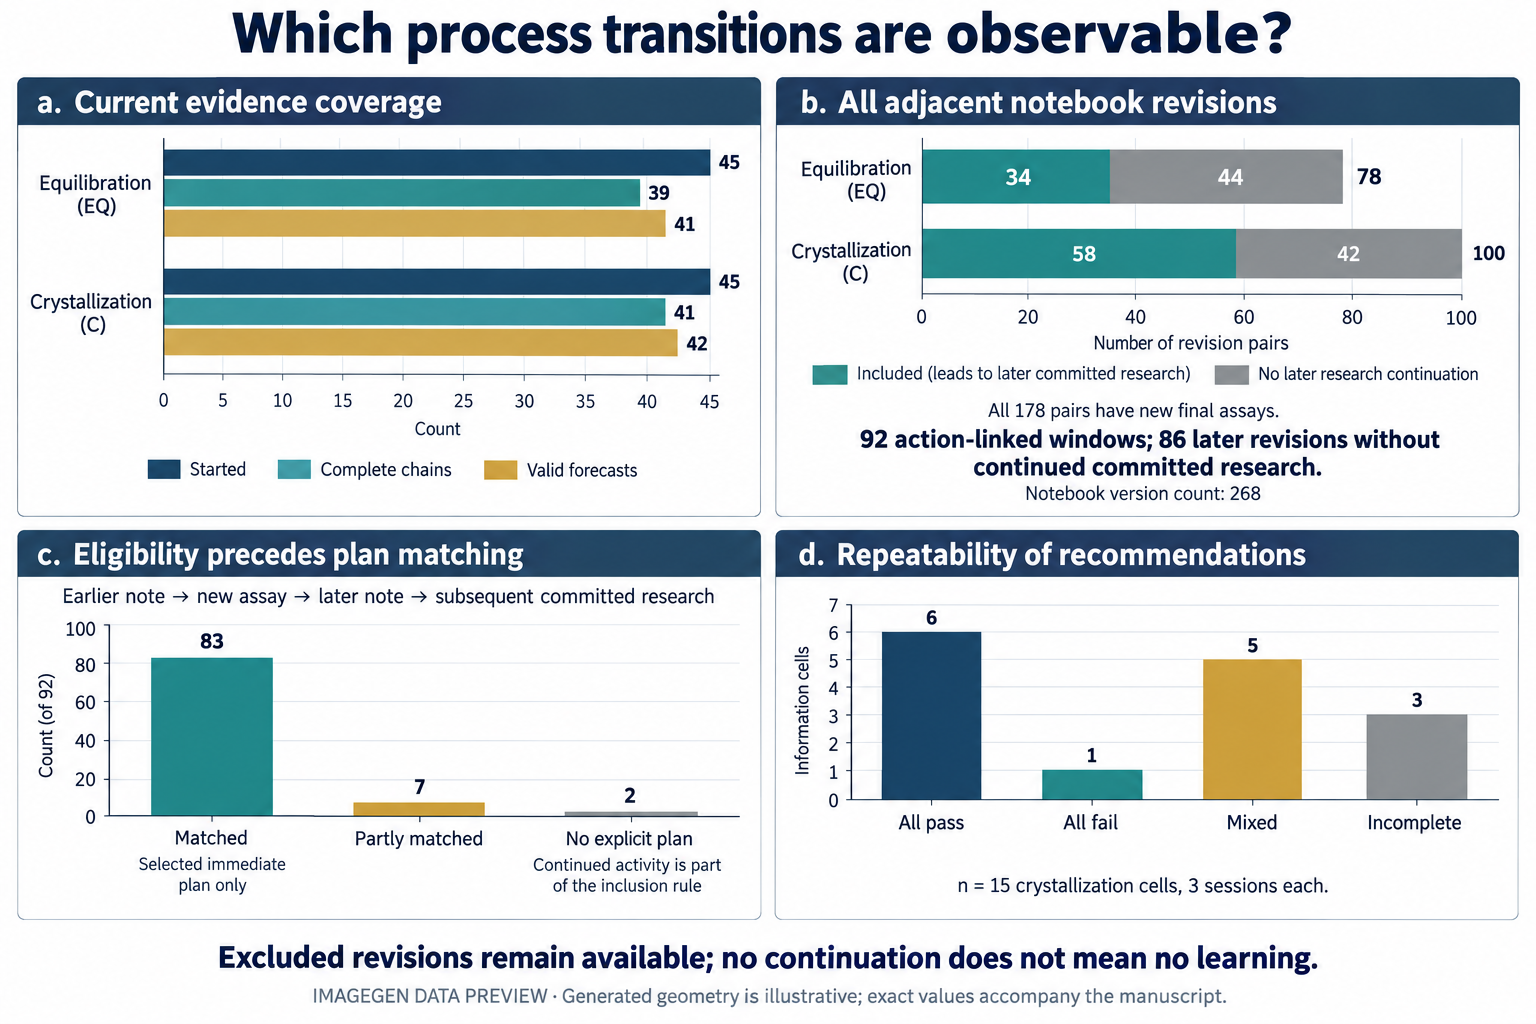
\includegraphics[width=\linewidth,height=.68\textheight,keepaspectratio]{../figures/preview-20261015/extended01.png}}
\caption{Extended Data Figure 1 \textbar{} Which process transitions are observable? ImageGen data preview. a, Current session coverage and valid forecasts. b, All 178 adjacent version pairs contain new assays: 34/78 equilibrium and 58/100 crystallization pairs also have a later committed research action, yielding 92 eligible windows. The remaining 86 revisions are retained without an action-linked code. c, The selected immediate plan is matched in 83 windows, partly matched in seven and absent in two. Eligibility precedes semantic matching but conditions the sample on continued activity; these counts do not measure learning success or cover every proposal. d, Across fifteen crystallization world-by-information cells with three sessions each, six are all-pass, one all-fail, five mixed and three incomplete. Generated geometry is illustrative.}
\end{figure}

\clearpage\begin{figure}[H]
\centering
\pandocbounded{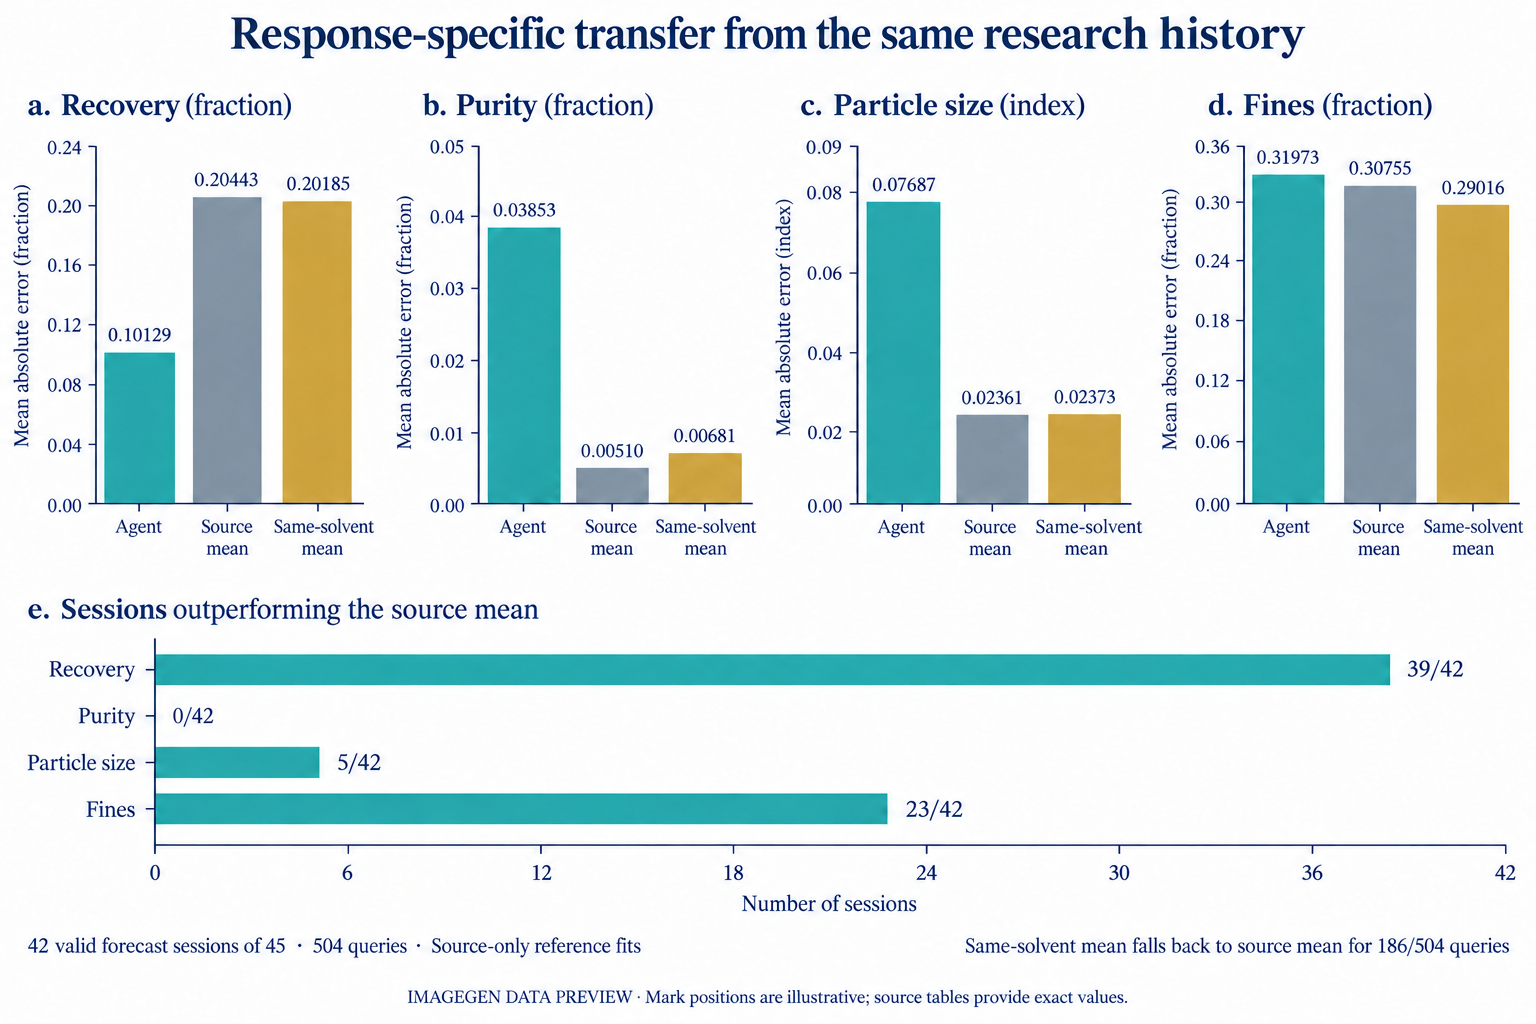
\includegraphics[width=\linewidth,height=.68\textheight,keepaspectratio]{../figures/preview-20261015/extended02.png}}
\caption{Extended Data Figure 2 \textbar{} Response-specific transfer from the same research history. ImageGen data preview. a--d, Agent forecasts and two source-only references are compared for recovery, purity, particle-size index and fines, retaining each response's own public scale. Particle size is the dimensionless index min(d50/250 micrometres, 1). e, Agent forecasts outperform the overall source mean in 39/42, 0/42, 5/42 and 23/42 sessions, respectively. The 42 valid corrected-crystallization sessions supply 504 forecast queries. Same-solvent means fall back to the overall mean in 186/504 queries and do not match thermal history or quantities. Neither reference is fitted to held-out truth. Generated geometry is illustrative; five-world-equal numerical errors are reported in the supplementary tables.}
\end{figure}

\clearpage\begin{figure}[H]
\centering
\pandocbounded{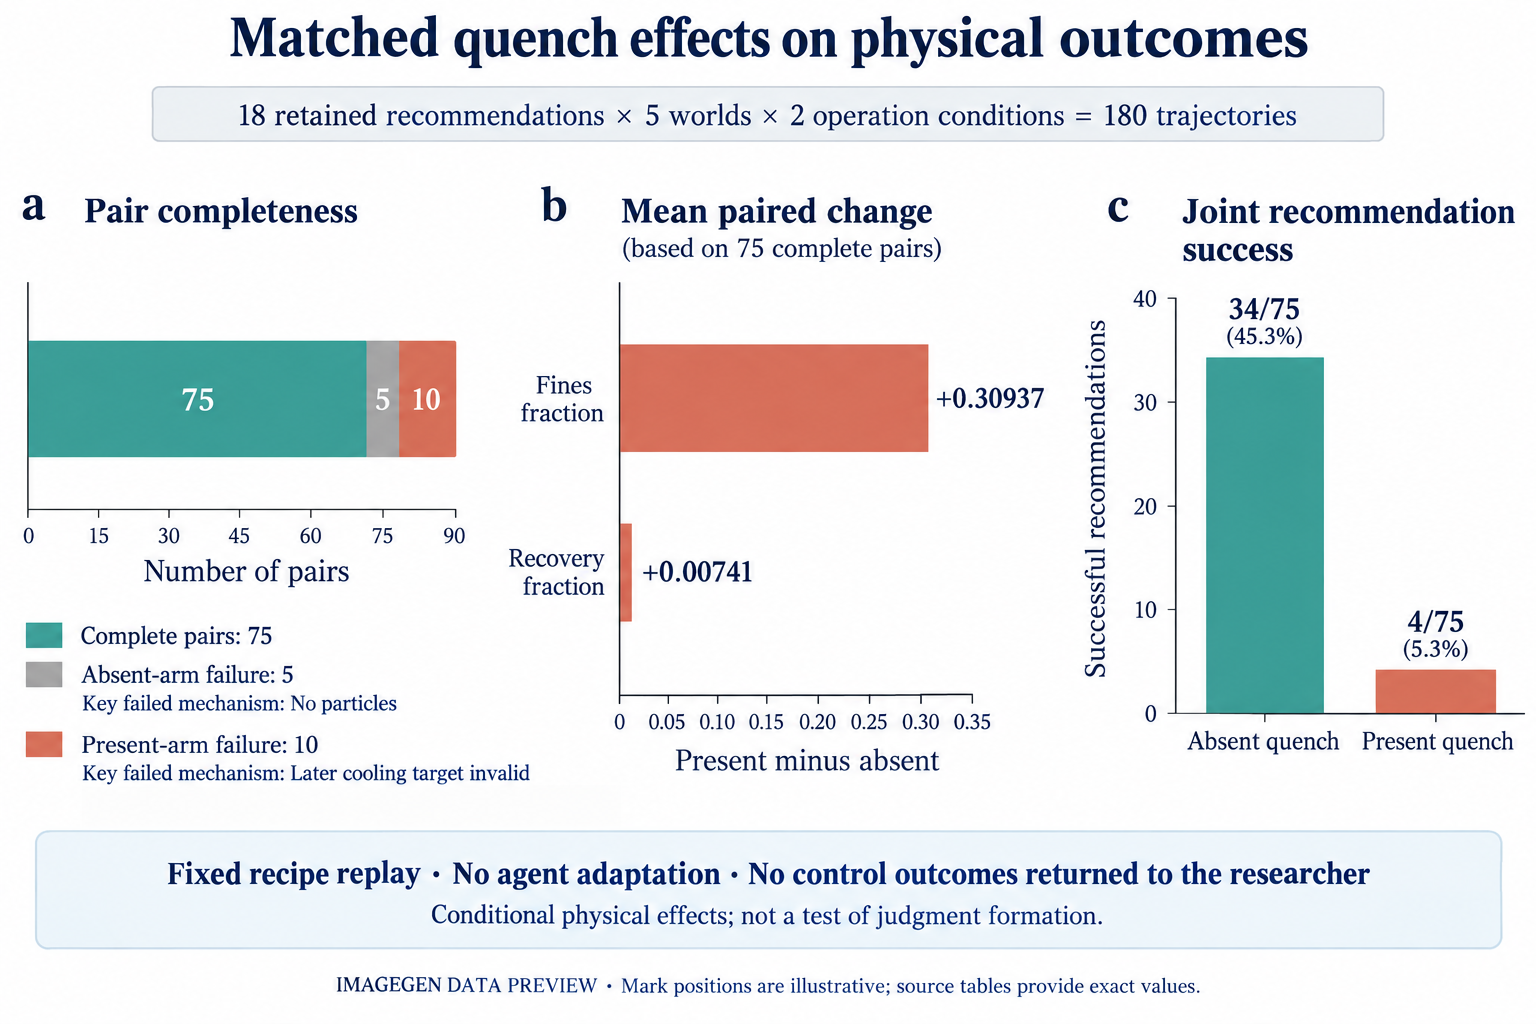
\includegraphics[width=\linewidth,height=.68\textheight,keepaspectratio]{../figures/preview-20261015/extended03.png}}
\caption{Extended Data Figure 3 \textbar{} Matched quench effects on physical outcomes. ImageGen data preview. Eighteen historical recommendations are replayed in five worlds with and without one quench operation, yielding ninety pairs and 180 trajectories. a, Seventy-five pairs yield both final assays; five absent arms lack particles and ten present arms invalidate a subsequent fixed cooling target. b, Complete-pair mean changes are +0.30937 in fines and +0.00741 in recovery. c, Joint success changes from 34/75 without quench to 4/75 with quench. These are conditional physical effects under the initial-charge recovery definition. The agent neither adapts nor receives control outcomes, so this intervention does not identify judgment formation. Generated geometry is illustrative and all failed pairs remain reported.}
\end{figure}

\end{document}
